\documentclass[12pt,a4paper]{book}
\title{My beautiful dissertation}
\author{Tobin South}
\date{\today}
\def\degree{Masters of Philosophy}
\def\discipline{Applied Mathematics}


% Any packages should go here
\usepackage{graphicx,natbib,thesis} 


\usepackage[colorlinks=true,linkcolor=blue,citecolor=blue,urlcolor=blue]{hyperref}       % hyperlinks
\usepackage{url}            % simple URL typesetting
\usepackage{booktabs}       % professional-quality tables
\usepackage{amssymb}  % special math fonts

% Colours
\usepackage{xcolor}
\definecolor{LeanLeft}{RGB}{49,102,158}
\definecolor{Left}{RGB}{159,201,103}
\definecolor{Center}{RGB}{150,103,159}
\definecolor{LeanRight}{RGB}{202,153,153}
\definecolor{Right}{RGB}{199,37,46}




% For align and more
\usepackage{amsmath}

% For subfigures
\usepackage{subcaption}

% For SVG
\usepackage{svg}
%\usepackage[clean]{svg}

% For multipage tables
\usepackage{longtable}

% Tikz
\usepackage{pgfplots}

%% Get width of thesis
%\usepackage{printlen}
%\printlength\textwidth

% For definitions
\usepackage{amsthm}
\theoremstyle{definition}
\newtheorem{definition}{Definition}[section]

\newtheorem{theorem}{Theorem}[section]
\newtheorem{corollary}{Corollary}[theorem]
\newtheorem{lemma}[theorem]{Lemma}

\newcommand{\definitionautorefname}{Definition}
\newcommand{\Theoremautorefname}{Theorem}
\newcommand{\lemmaautorefname}{Lemma}


\theoremstyle{remark}
\newtheorem*{remark}{Remark}

% Make QED symbol black square
\renewcommand\qedsymbol{$\blacksquare$}


%% Add spacing to tables 
%\usepackage{array}
%\setlength\extrarowheight{2pt} % or whatever amount is appropriate

%% Add spacing to table captions
%\usepackage{caption} 
%\captionsetup[table]{skip=10pt}



\newcommand{\todo}[1]{{\color{red}[[TODO: {#1}]]}}
\newcommand{\lm}[1]{{\color{orange}[[LM: {#1}]]}}
\newcommand{\mr}[1]{{\color{blue}{MR: {#1}}}}
\newcommand{\ts}[1]{{\color{purple}[[TS: {#1}]]}}
\newcommand{\tocite}[1]{{\color{red}[[CITE: {#1}]]}}


\begin{document}
%\frontmatter
%
%\maketitle
%
%% Make the following tables
%\tableofcontents
%\listoftables
%\listoffigures
%
%% Import the various things
%%!TEX root = ../thesis.tex
\chapter{Signed statement}
{\parindent=0pt\parskip=4ex

%
%  Check the University website for the current statements.  The ones below are from 
%    http://calendar.adelaide.edu.au/aprhdr/2016/specifications-thesis
%  and valid for 2016
%
%  The second one is for when you are using material that is already published.  
%


%4.1	For a thesis that does not contain work already in the public domain.

% I certify that this work contains no material which has been accepted for the award of any other degree or diploma in my name in any university or other tertiary institution and, to the best of my knowledge and belief, contains no material previously published or written by another person, except where due reference has been made in the text. In addition, I certify that no part of this work will, in the future, be used in a submission in my name for any other degree or diploma in any university or other tertiary institution without the prior approval of the University of Adelaide and where applicable, any partner institution responsible for the joint award of this degree.

% I give consent to this copy of my thesis, when deposited in the University Library, being made available for loan and photocopying, subject to the provisions of the Copyright Act 1968.

% I also give permission for the digital version of my thesis to be made available on the web, via the University's digital research repository, the Library Search and also through web search engines, unless permission has been granted by the University to restrict access for a period of time.

%
%%4.2	For a thesis that contains publications.
%
I certify that this work contains no material which has been accepted for the award of any other degree or diploma in my name, in any university or other tertiary institution and, to the best of my knowledge and belief, contains no material previously published or written by another person, except where due reference has been made in the text. In addition, I certify that no part of this work will, in the future, be used in a submission in my name, for any other degree or diploma in any university or other tertiary institution without the prior approval of the University of Adelaide and where applicable, any partner institution responsible for the joint-award of this degree.

I acknowledge that copyright of published works contained within this thesis resides with the copyright holder(s) of those works.

I also give permission for the digital version of my thesis to be made available on the web, via the University’s digital research repository, the Library Search and also through web search engines, unless permission has been granted by the University to restrict access for a period of time.


Signed: \dotfill\quad 
Date: \dotfill

}


%%!TEX root = ../thesis.tex
\chapter{Acknowledgements}
\label{ch:acknowledgements}

%%!TEX root = ../thesis.tex
\chapter{Dedication}
\label{ch:dedication}

%%!TEX root = ../thesis.tex
\chapter{Abstract}
\label{ch:abstract}

Chapter~\ref{ch:intro} introduces 




\newpage

\mainmatter

% Import the chapter files
%!TEX root = ../thesis.tex
\chapter{Background \label{ch:background}}

\todo{Introduction to background}
Information theory, what is it, why do we use it
Networks, why
Natural language processing


\subsection{Information Theory}

\subsubsection{Entropy}
Entropy is a measure of the uncertainty of a random variable. In the context of information theory, this is defined by \autoref{eq:shannon}, often refereed to as Shannon entropy, named after Claude Shannon for his work in 1948 studying the quantiles of information in transmitted messages~\todo{cite Claude shannon 1948}. The definitions hereafter are sourced from Elements of Information Theory by Thomas and Cover \tocite{elements of information theory} 

\begin{definition}[Shannon Entropy]
	Let $X$ be a discrete random variable with alphabet $\mathcal{X}$ and probability mass function $p(x) = P(X = x), x \in \mathcal{X}$.
	The entropy $H(X)$ of the discrete random variable X, measured in bits, is 
	\begin{equation}\label{eq:shannon}
	H(X)=-\sum_{x \in \mathcal{X}} p(x) \log_2 p(x)
	\end{equation}
\end{definition} 

The entropy of the random variable is measured in bits. A bit can have two states, typically 0 or 1. The entropy of a random variable is the number of bits on average that is required to describe the random variable in question. To measure the entropy in bits, we use a logarithm of base 2, and all logarithms throughout this work are assumed to be in based 2, unless otherwise specified.

To give a typical example of entropy, if a fair coin is tossed there are two equally probable outcomes, giving an entropy of 1 bit. Further, we use the convention of $0\log 0 = 0$, which sensibly means that adding a state with 0 probably to the random variable does not change it's entropy.

\begin{remark}[Suprise]
	The entropy of the random variable X can also be described in terms of the expected surprise, where the surprise of a state is $\log \frac{1}{p(x)}$.
	\begin{equation}
		H(X) = \mathbb{E} \left[ \frac{1}{p(x)} \right]
	\end{equation}
\end{remark}	



\todo{add some filler}


\begin{lemma}
	The entropy of a random variable is strictly non-negative, $H(X) \geq 0$.
\end{lemma}

\begin{proof}
	$0 \leq p(x) \leq 1$ which implies that $log \frac{1}{p(x)} \geq 0$,
	hence the sum of products of strictly non-negative terms will always be non-negative. 
\end{proof}

\todo{add some filler}

\subsubsection{Joint Entropy and Conditional Entropy}

Above we worked with a single random variable. To extend this we introduce a second discrete random variable $Y$. Using this, we extend the one dimensional entropy to joint entropy. 

\begin{definition}[Joint Entropy]
	The joint entropy $H(X,Y)$ of a pair of discrete random variables $(X,Y)$ with a joint distribution $p(x,y)$ and state spaces $(\mathcal{X}, \mathcal{Y})$
	\begin{equation}\label{eq:jointentropy}
	H(X, Y)=-\sum_{x \in \mathcal{X}} \sum_{y \in \mathcal{Y}} p(x, y) \log p(x, y)
	\end{equation}
\end{definition}

From our definition of entropy and the law of total probability we can create a notion of conditional entropy.

\begin{definition}[Conditional Entropy]
	The conditional entropy $H(X|Y)$ of two discrete random variables $X$ and $Y$ is defined as, 
		\begin{align}
		H(X | Y)&=\sum_{y \in \mathcal{Y}} p(y) H(X |Y=y) \\
		&=-\sum_{y \in \mathcal{Y}} p(y) \sum_{y \in \mathcal{Y}} p(x | y) \log p(x | y) \\ 
		&=-\sum_{y \in \mathcal{Y}} \sum_{y \in \mathcal{Y}} p(x, y) \log p(x | y) \\ 
		&=-E \log p(X | Y)
		\end{align}
\end{definition}


Subtly different from the \emph{conditional entropy} is the \emph{cross entropy}. Whereas the \emph{conditional entropy} is the amount of information needed to describe $X$ given the knowledge of $Y$, the \emph{cross entropy} is the amount of information needed to describe $X$ given a optimal coding scheme built from $Y$. 

\begin{definition}[Cross Entropy]\label{def:crossentropy}
	The cross entropy $H_{\times} (q|p)$ between two probability distributions, defined over the same state space, $p$ nd $q$ is defined as, 
	\begin{equation}
	H (q||p)= - \sum_{x} p(x) \log {q(x)}
	\end{equation}
\end{definition}

Although cross entropy has the common notation $H(X, Y)$, in this thesis we will use an alternative $H(X||Y)$, reminiscent if the Kullback–Leibler divergence in~\autoref{eq:kldivergence} below, so as to not confuse the cross entropy with the above join entropy~\autoref{eq:jointentropy} of the same notation.



\begin{remark}
	Importantly, note that $H(X|Y) \neq  H(Y|X)$ and $H(q||p) \neq H (q||p)$, both properties we will exploit later.
\end{remark}


\subsubsection{Distances}
We can extend these ideas to explore a notion of distance between probability distributions. Kullback–Leibler divergence is a measure of the inefficiency if one were to assume that a distribution is $p$ when the true distribution is $q$.

\begin{definition}[Kullback–Leibler divergence]
	The Kullback–Leibler divergence (also called relative entropy), $D(p \|q)$,  between two probability distributions $p(x)$ and $q(x)$ is,
	\begin{align} \label{eq:kldivergence}
		D(p \| q) &=\sum_{x \in \mathcal{X}} p(x) \log \frac{p(x)}{q(x)} \\ 
					 &=E_{p} \log \frac{p(X)}{q(X)} 
	\end{align}
\end{definition}

Again, we use the convention that  $0 \log \frac{0}{0} = 0 $ and $p \log \frac{p}{0} = \infty $. 


Conveniently, we can also express the Kullback–Leibler divergence in terms of the cross entropy.
\begin{lemma}
		\begin{equation}
		D(p \| q) = H_p(q) - H(p) 
		\end{equation}
\end{lemma}
\begin{proof}
	\begin{align}
		D(p \| q) &=\sum_{x \in \mathcal{X}} p(x) \log \frac{p(x)}{q(x)} \\
		 &= \sum_{x \in \mathcal{X}} p(x) \log p(x)    -     \sum_{x \in \mathcal{X}} p(x) \log q(x)\\
		 &= -H(p)   +    H(q||p)\\
	\end{align}
\end{proof}

The Kullback–Leibler divergence has two difficulties; It's not symmetrical and it can return infinite values. Jensen–Shannon divergence builds from the Kullback–Leibler divergence to solve these problems to a symmetric, finite comparison between probability distributions. 

\begin{definition}[Jensen–Shannon divergence]
 The Jensen–Shannon divergence between two probability distributions $p(x)$ and $q(x)$ is,
	\begin{equation}
	\operatorname{JSD}(p \| q)=\frac{1}{2} D(p \| m)+\frac{1}{2} D(q \| m)
	\end{equation}
	using a mixture of the distributions, 	$m=\frac{1}{2}(p+q)$.
\end{definition}


\begin{remark}
	The square root of the Jensen–Shannon divergence provides a metric, often referred to as Jensen–Shannon distance.
\end{remark}

\ts{define metric?}


\ts{add mutual information}

\ts{add variation of information}

\ts{add diagram}


\subsubsection{Entropy Rates}

Entropy rate of a stochastic process describes the amount of information required to describe the future state of a process, conditioned on the information in the history of the process.

"The entropy rate is almost surely an asymptotic lower bound on the per-symbol description length when the process is losslessly encoded" \tocite{Some asymptotic properties of entropy of a
	stationary ergodic data source with applications to data compression,}

\begin{definition}[Entropy Rate]\label{def:entropyrate}
	Let  $\mathcal{X}= \{ X_i \}$ be a stochastic ergodic process with a finite alphabet, where $X_i^j$ denotes a subsequence of the process $(X_{i}, X_{i+1}, \ldots, X_{j})$.
	The entropy rate can be defined as,
	\begin{equation}\label{eq:entropyrate}
	H(\mathcal{X})=\lim _{n \rightarrow \infty} H\left(X_{n} | X_{n-1}, X_{n-2}, \ldots, X_{1}\right)
	\end{equation}
	Which, on the assumption of stationary, can be expressed as,
	\begin{equation}
	H(\mathcal{X})=\lim _{n \rightarrow \infty} \frac{1}{n} H\left(X_{1}, X_{2}, \ldots, X_{n}\right)
	\end{equation}
\end{definition}

While this notion of entropy rate provides a valuable theoretical tool, calculating it for real examples can prove difficult, and often impossible given data. In \autoref{ch:crossentropy} we will explore a method of estimating a similar quantity.



\subsubsection{Predictability}

Predictability is the probability $\pi$ that an theoretical predictive algorithm could predict the next state of a process correctly, this often be difficult to obtain. However, an upper bound, $\pi \leq \pi^{max}(S,N)$, is possible through the use of Fano's inequality~\cite{fano_transmission_1961}. For a process with $\pi^{max} = 0.3$, at best we could hope to predict this process correctly 30\% of the time, no matter how good our predicative algorithm~\cite{song_limits_2010}.


\begin{definition}[Maximal Predictability]
For a process $X$ with entropy $H(X)$, Fano's inequality in the context of our maximal predictability gives,
\begin{equation}
H(X) = H(\pi^{max}) + (1 - \pi^{max}) \log (|\mathcal{X}| - 1)
\end{equation}
\end{definition}

The entropy of the maximal predictability $H(\pi^{max})$ is substituted with the binary entropy function~\cite{song_limits_2010},   
\begin{equation}
H(\pi^{max}) = -\pi^{max} \log(\pi^{max}) - (1 -  \pi^{max}) \log(1 - \pi^{max}).
\end{equation}

Which finally gives us a form that can be solved numerically for the fundamental limit of the process' predictability, $\pi^{max}$,
\begin{equation}\label{eq:predict}
-H(X)  = \pi^{max} \log(\pi^{max}) + (1 -  \pi^{max}) \log(1 - \pi^{max}) - (1 - \pi^{max}) \log (|\mathcal{X}| - 1).
\end{equation}


Throughout this thesis, maximal predictabilities will found by solving \autoref{eq:predict} using the Powell's conjugate direction method, implemented in python using SciPy~\cite{virtanen_scipy_2019}, with a starting estimate for the root at $\pi^{max}=0.5$.



% cross predictaibility
We extend this notion of maximal predictability of a process, to create a cross predictability using cross entropy~\autoref{def:crossentropy}.
\todo{more}



\subsection{Networks}

\todo{go through Newman networks and state a bunch of definitions}









\subsection{Natural Language Processing}

\ts{introduce in here the notion that we're interested in text and NLP is a fundamental building block of understanding it}

Natural language processing (NLP) is the area of study in which 'natural' human language is examined via machine. Natural language refers to either spoken or written language, designed to be understandable to a human listener or reader. This language is not explicitly designed to be machine understandable, and machine comprehension of this language is a challenging problem \tocite{cite: the challenges of NLP}.

NLP is a broad term covering many models and techniques to computationally extracting meaningful information from text, ranging from the simple extraction of individual words, to the extraction of deeper semantic meaning. 

Early work in NLP focused around simple grammatical rules and small vocabularies, such as the work of Georgetown-IBM \tocite{cite: John Hutchins. From first conception to first demonstration: the nascent years of machine translation, 1947–1954. a chronology. Machine Translation, 12(3):195–252, 1997.} to translate 60 sentences from Russian to English in 1954. With the rapid increase in computational power and digital text corpuses, modern NLP has focused or deeper challenges of extracting meaning from text with tools such as Word2Vec \tocite{cite: word to vec} or deep learning methods such as Google's BERT \tocite{cite: BERT}.

These methods face a daunting challenge, language is not only complex and often duplicitous, but contextual and ever-changing. \todo{end better}

\subsubsection{Tokenisation} 





%!TEX root = ../thesis.tex
\chapter{The one with data and BOW\label{ch:dataandBOW}}

The main source of data for analysis is draw from the Twitter accounts of news-media organisations. In the 1950s, the widespread popularity of household television allowed TV broadcasting to become the primary tool for influencing public opinion in developed nations~\todo{cite: Diggs-Brown, Barbara (2011) Strategic Public Relations: Audience Focused Practice p.48}.  This was a shift from a population that \emph{listened} to radio news, to a population that \emph{watched} news. 

The even more rapid rise of mobile internet and social media sites in the last two decades has caused another shift. No longer just a population that watch news at fixed time, or read regularly scheduled newspapers; the conveniences of the modern developed world allow individuals to consume news anytime, anywhere. As of 2019, 55\% of US adults get their news from social media either `often' or `sometimes'~ and 88\% state that `social media companies have at least some control over the mix of news people see'~'\cite{shearerAmericansAreWary2019}.

Given the importance of a free press and the role of social media sites in the delivery of news, this work aims to study the news on social media. To begin this task, we first define some common terms for clarity.

\begin{definition}[Social media]
	The platforms used to consume information by individuals in the public. E.g. Twitter, Facebook, Reddit.
\end{definition}

\begin{definition}[News-media]
	The organisations that are producing information about a broad range of current events and sharing that information with the public.
\end{definition}

\begin{definition}[News]
	The \emph{content} produced by news-media organisations. 
\end{definition}

\section{Data}

Using the media analysis source AllSides\footnote{www.allsides.com}, a collection of news-media organisations was found. The purpose of AllSides is to provide a public analysis of political leanings of news sources~\todo{cite: https://www.allsides.com/media-bias/media-bias-ratings}, and to aggregate news allowing consumers to view articles from different sides of the political spectrum. Each news source is labelled into one of 5 categories, Left, Lean Left, Center, Lean Right, or Right. Any news source the ratings are determined internally using `blind surveys of people across the political spectrum, multi-partisan analysis, editorial reviews, third party data, and tens of thousands of user feedback ratings'~\todo{cite: same as above}. News sources are only assigned to a single category, but do have an attached confidence rating.

From the website, a list of possible news sources was collected on February 1st, 2019. In this collection was organisation names, political bias', the number of user feedback ratings of the political bias, and, if available, the twitter handles associated with those sources. These collected news sources were broad, containing not just news-media organisations but authors, pundits and think tanks. 

To select an appropriate set of news-media organisation an examination and filtering process was undertaken. A source was only considered if it was a organisation (not an individual), that produced news content of a diverse range of topics. Many news sources were connected to think tanks or opinion groups, and only created news of a single topic or campaign. Further, if an news-media organisation has no twitter account or had less than 10,000 followers (a low bar in the social media world), then it was removed from the pool. This mainly removed inactive organisations and news organisation from small rural towns. Finally, a single sources was removed as it was not in English, and a single source was removed as it was the smaller sister site that had all content as a subset of it's larger site.  The result of this filtering process is 174 news-media organisations and associated twitter accounts and categorised political bias'.  A list of all news-media organisations under analysis can be seen in \cite{app:accounts} and all removed sources and the removal justification can be seen in \todo{appendix of removals}.

%twitter collection
Using the Twitter user handles associated with each of the news-media organisations, the history of all tweets for each account was collected using the Twitter application programming interface (API)\footnote{https://developer.twitter.com/en/docs}. Of interest in this work are the tweets each news organisation tweeted between January 1st, 2019 to January 1st, 2020. 

% removal of inactive twitter accounts
Using this collection method a total of 3,221,769 tweets were collected from the 174 news-media organisation official Twitter accounts. 

% location diverstity but america



60054638 words




% plots of the daily twitter activities of each news organition of 

% make a comment amount average activity levels (number of tweets??)





%!TEX root = ../thesis.tex
\chapter{Entropy rate estimation}\label{ch:crossentropy}

\epigraph{\em ``Semantic aspects of communication are irrelevant to the engineering problem.''}{Claude Shannon, {\em A Mathematical Theory of Communication}, 1948}

Extracting information flows is a problem deeply rooted in information theory. To examine these flows requires tools to quantify and measure this information in the form of natural language. As discussed in \autoref{ch:background}, the words used to construct language have no qualitative meaning in the context of the numerical analysis. Thus the tools are comparative in nature. Indeed, information theory has been used extensively to compare properties of information in language~\cite{shannon_prediction_1951,cover_convergent_1978,brown_estimate_1992}. 

In this chapter, we extend this philosophy in two key ways. We introduce a non-parametric entropy rate estimator and check its assumptions using real data. We then generalise this entropy rate to a cross entropy rate, developing a tool for analysing information flows. These new estimators are then made into a high speed open-source package which is applied to our news data. 

\section{Entropy rate estimation}

Recall \autoref{def:entropyrate} of the entropy rate of a stochastic process. While a useful theoretical tool, this can be very difficult to compute, requiring knowledge of the joint entropy for an infinite set of realisations.

To overcome this, we seek a way to estimate the entropy of the process from a known sequence of data. In 1998 Kontoyiannis \emph{et al.}~\cite{kontoyiannis_nonparametric_1998} proved the convergence of a non-parametric entropy estimator for stationary processes.

\begin{definition}[Kontoyiannis Entropy Rate] \label{def:Kontoyiannis}
	For a discrete valued stochastic process $\mathcal{X} = \{X_i\}_{i=0}^N$, with $N$ realisations, the entropy rate is given by,
	\begin{equation}\label{eq:entropy:Kontoyiannisdef}
		H(\mathcal{X}) = \lim_{N\to \infty}\frac{N \log N }{\sum_{i=0}^N \Lambda_{i} },
	\end{equation}
	where  $\Lambda_{i}$ is the length of the shortest subsequence starting at position $i$ that does not appear as a contiguous subsequence in the previous $i$ symbols, $X_{0}^{i} = \{X_k\}_{k=0}^i $. This can also be obtained by adding 1 to the longest match-length, 
	 \begin{equation}\label{eq:entropy:lambda}
	  \Lambda_{i}=1+\max \left\{\ell: X_{i}^{i+\ell}=X_{j}^{j+\ell}, 0 \leq j \leq N-i, 0 \leq \ell \leq N - i - j \right\}.
	 \end{equation}
\end{definition}

%<lit review>
This idea of using matched sub-sequences of text draws from the original work by Lempel and Ziv~\cite{ziv_universal_1977} in compression algorithms. These algorithms attempt to compress a sequence down into the smallest possible representation, which at perfect efficiency would be the entropy, $H$. However these universal coding algorithms have no universal rate of convergence~\cite{shields_universal_1993, shields_universal_1995} and in practice other approaches are often employed, tailored to the specific application at hand.

The idea of an entropy estimator based on match lengths was originally put forward by Grassberger~\cite{grassberger_estimating_1989} and proved consistent for independent and identically distributed (i.i.d.) processes and mixing Markov chains~\cite{shields_entropy_1992}, stationary processes~\cite{kontoyiannis_prefixes_1994} and more generally for random fields~\cite{quas_entropy_1999}.


Wyner and Ziv~\cite{wyner_asymptotic_1989} showed that for every ergodic process the match length $\Lambda_{n}$ grows like $\frac{\log{n}}{H}$ in probability.  Extending from this notion Kontoyiannis \emph{et al.} showed the convergence of \autoref{eq:entropy:Kontoyiannisdef} in stationary ergodic processes using the match-length $ \Lambda_{i}$. This match-length in \autoref{eq:entropy:lambda} can be seen as the length of the next phrase to be encoded in the sliding-window Lempel–Ziv algorithm.

%<match lengths>
Conceptually, this match-length is simple. \autoref{fig:entropy:matchlength} shows the calculation of two match-lengths at different time points of a line from Green Eggs and Ham by Doctor Seuss. At each index $i$, the elements immediately proceeding ($i, i+1, i+2, \dots$) are compared to the history of elements before $i$. The matches of length $k$ are found such that the elements from $j$ to $j+k$ perfectly match the elements from $i$ to $i+k$, for any $j<i$ where $k$ is then maximised. This search only considers the length of the match, regardless of its location in the history. 

\begin{figure}[!htbp]
	\centering
	\includestandalone[width=\textwidth]{chapter2/figs/tikz/lambda_count}
	\caption{An example calculation of the match-length based $\Lambda_i$ applied to a words in a line of text from Green Eggs and Ham by Doctor Seuss. The {\color{blue}blue texts} are words which have been matched from past to the future. As $i$ changes, the longest match length possible starting at index $i$ will change.\label{fig:entropy:matchlength}} 
\end{figure}
%</match lengths>

Even before its formalisation by Kontoyiannis \emph{et al.}, similar estimators had appeared in the literature applied to experimental data to determine the entropy rates of processes~\cite{chen_using_1993, chen_fast_1995, farach_entropy_1995, juola_what_1997}.
%</lit review>

% Final note
Moving forward we will assume any any discussion of the \emph{entropy rate} of a single process is assumed to be the \emph{Kontoyiannis entropy rate} of that process, unless otherwise stated.


% ASSSUMPTIONS
\section{Assumptions of entropy rate estimation}

The proof of convergence of this entropy rate places some limits on the process of investigation. In particular, three assumptions are made for convergence: ergodicity, stationarity and the Doeblin Condition (DC).

The Doeblin Condition is a reasonably weak condition, but is fundamental in the proof of the convergence. Simply put, the DC requires that after an arbitrary $r$ time steps, every state is possible again with positive probability~\cite{kontoyiannis_prefixes_1994}. More formally, the definition is as follows.

\begin{definition}[Doeblin Condition (DC)]
	There exists an integer $r\geq 1$ and a real number $\beta \in(0,1)$ such that, for all states $x_{0} \in \mathcal{A}$, 
	$$P\left\{X_{0}=x_{0} \mid X_{-\infty}^{-r}\right\} \geq \beta, $$ 
	with probability one. 
\end{definition}

Fortunately, as Kontoyiannis \emph{et al.} themselves state, the DC is ``certainly satisfied by natural languages''~\cite{kontoyiannis_nonparametric_1998}. 

In contrast, the assumptions of ergodicity and stationarity are  harder to confirm. A long-standing assumption of information theory is that natural language can be modelled by a stationary process~\cite{shannon_mathematical_1948, shannon_prediction_1951, cover_elements_2012}. The assumption, while flawed, has a long precedent and we use it again in this work.

Much of the literature including the work of Kontoyiannis assume ergodicity of natural language, however some suggest that language should be modelled by a \emph{strongly nonergodic} stationary process~\cite{debowski_is_2018}. In brief, this contention is founded upon the idea that any given collection of text, such as a book, has a topic containing a small finite subset of words. Which suggests that its text cannot explore the full state space of language. While well founded, our interest is not to look at the entropy rate of the English language as a whole, but rather to look at the entropy rate of individual text streams, which can all explore the state space of news under consideration. As such, the assumptions of ergodicity and stationarity appear justified in the context of the problem.


%<Convergence>
\subsubsection{Convergence}
With the assumptions of the proof addressed, the challenge of entropy rate estimation convergence needs to be examined. The entropy rate defined in \autoref{eq:entropy:Kontoyiannisdef} is based upon an infinite set of data. In reality, we have finite data, and need to examine the convergence of a modified estimator.

\begin{definition}[Kontoyiannis Entropy Rate Estimator] \label{def:Kontoyiannisestimate}
	The Kontoyiannis Entropy Rate in \autoref{def:Kontoyiannis} can be estimated on a finite stochastic process $\mathcal{X} = \{X_i\}$, with $N$ realisations, by
	\begin{equation}\label{eq:estimate}
		\hat{h} = \frac{N \log N }{\sum_{i=0}^n \Lambda_{i} },
	\end{equation}
	where  $\Lambda_{i}$ is, as earlier, the length of the shortest subsequence starting at position $i$ that does not appear as a contiguous subsequence in the previous $i$ symbols $X_{0}^{i}$.
	 \begin{equation}
	  \Lambda_{i}=1+\max \left\{\ell: X_{i}^{i+\ell}=X_{j}^{j+\ell}, 0 \leq j \leq N-i, 0 \leq \ell \leq N - i - j \right\}.
	 \end{equation}
\end{definition}

To examine the convergence of this estimator, a model of language can be used to generate sequences of text, upon which we can estimate the entropy rate.

%<Zipf convergence>
\begin{figure}[!htbp]
\centering
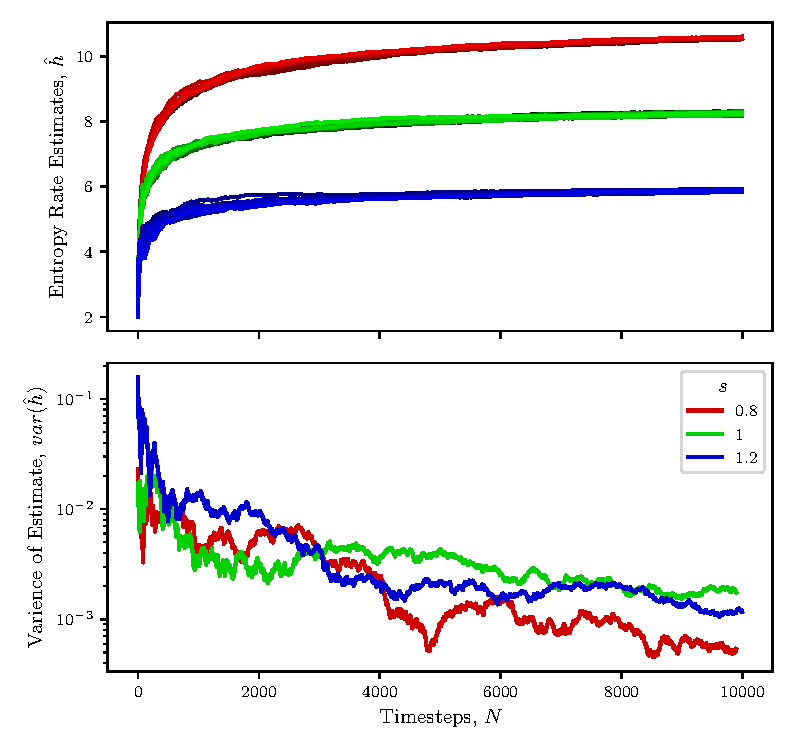
\includegraphics[width=\textwidth]{chapter2/figs/Zipf_entropy_convergence.pdf}
\caption{Convergence of the Kontoyiannis entropy rate estimator on sequences of i.i.d. Zipf distribution realisations with varying Zipf distribution rates, $\alpha$. \label{fig:entropy:zipfconvergence}}
\end{figure}


\autoref{fig:entropy:zipfconvergence} shows the convergence of the estimator for a set of i.i.d. realisations of a Zipf distribution. As discussed in \autoref{sec:textgeneration}, the Zipf distribution is a common tool for generating simple text due to its similarity to the power-law distributions of vocabulary seen in real corpora. The Zipf distribution can be used with a number of scaling parameters, $\alpha$, where larger scaling parameters tighten the distribution, reducing the observed vocabulary size of the sequence and hence the entropy. 

Sequences are generated with 30,000 i.i.d. elements drawn from a Zipf distribution and the entropy rate of estimate of the process is calculated at each timestep between 1 and 30,000 using \autoref{eq:estimate} applied to only the elements before that timestep. Estimates of entropy start very low when few elements are available and rapidly rise as new elements add complexity. Within the first few hundred timesteps entropy estimates can vary between timesteps as new elements are added matching or not-matching previous elements. This is reflected in the high variance between entropies estimates for Zipf process with the same scaling parameter in these early stages. As the number of timesteps included reaches 5000 to 7500 the apparent bias from the asymptotic rate and variance of the estimates are significantly reduced and begin plateauing. 

As more timesteps are added, the estimator continues to converge to the asymptotic entropy and the variance between estimates continues to reduce. High complexity sequences take longer to converge to this entropy, but achieve suitably small levels of bias and variance within 15,000 timesteps even for high entropy sequences. This is an important finding given the speed of calculating these estimates. The algorithm to calculate the match-lengths needed for estimating the entropy is $O(N^3)$ time complexity for the number of included timesteps $N$. As a result, calculations are extremely slow as the number of timesteps gets large. When performing simulations a parsimonious choice of simulation length is advantageous in allowing multiple simulations to be run. Hence, for Zipf distributions a simulation length of 15,000 is deemed sufficient for convergence to the entropy.
%</Zipf convergence>


%<Zipf real entropy>
To confirm the validity of this approach, we can examine the known entropy rate of the Zipf processes. As proved in \autoref{sec:entropyrate}, the entropy rate of an i.i.d. process is simply the entropy of each element. In the case of a Zipf distribution the distribution has entropy\footnote{
	Proof: The probability of a word of rank $k$ being selected from a pool of $V$ elements using scaling parameters $\alpha$ is $(k^\alpha H_{V,\alpha})^{-1}$. Hence, the entropy of each individual element is $\sum_{k=1}^V  (k^\alpha V_{V,\alpha})^{-1} \ln\left( (k^\alpha V_{V,\alpha})^{-1} \right)$. Using $H_{V,\alpha} = \sum_{k=1}^V \frac{1}{k^\alpha}$, this can be rearranged to $\frac{\alpha}{H_{V, \alpha}} \sum_{k=1}^{V} \frac{\ln (k)}{k^{\alpha}}+\ln \left(H_{V, \alpha}\right)$. 
}, 
\begin{equation}
	\frac{s}{H_{V, \alpha}} \sum_{k=1}^{V} \frac{\ln (k)}{k^{\alpha}}+\ln \left(H_{V, \alpha}\right),
\end{equation}
where $H_{V,\alpha}$ is the $V$th generalized harmonic number defined by, 
$$H_{V,\alpha} = \sum_{k=1}^V \frac{1}{k^\alpha},$$
and $V$ is the size of the state space of the Zipf distribution. Many approaches to calculating this entropy use the asymptotic entropy as $V \to \infty$. This draws on the result that $\lim_{V\to \infty} H_{V,s} = \zeta(\alpha)$, where $\zeta$ is the Riemann zeta function. While this asymptotic approach works well for numbers well above 1, the Riemann zeta function diverges to infinity at $\alpha \to 1$. As such, the analytic entropy degenerates as $\alpha \to 1$ and is poorly defined for $\alpha < 1$. In contrast, using a finite choice of $V$ results in well defined processes and entropies for all $\alpha >0$. A choice of $V=199,338$ is made to match the observed total vocabulary size seen in the news-media Twitter data as explored in \autoref{sec:vocabsizes}. For high values of $\alpha$, the two asymptotic and finite entropies are very close (\emph{e.g}, for $\alpha=1.5$ the entropies are 3.18158 and 3.18368 respectively), and only differ significantly as $\alpha$ approaches 1. This finite entropy calculation allows the model to more accurately match the Zipf scaling parameters fitted to real text data, which are often closer to or below~1~\cite{williams_text_2015}.

% <Simulations>
Using simulations of the Zipf process for a variety of values of the scaling parameter $\alpha$, we compare how the estimated entropy rate compares to the `true' entropy rate as calculated above. In \autoref{figs:entropy:convergencetotruth} simulations are run for values of $\alpha$ in the range [0.01, 2] with increments of 0.01. 
High values of $\alpha$ in this range have a progressively lower entropy, as the skewness of the distribution becomes more extreme. This distribution results in a large number of realisations of low rank words creating repeated sequences which lower both the analytic entropy rate and the entropy rate estimate. Values above 2 reduce the entropy rate in vanishingly smaller increments. 

\begin{figure}[!htbp]
\centering
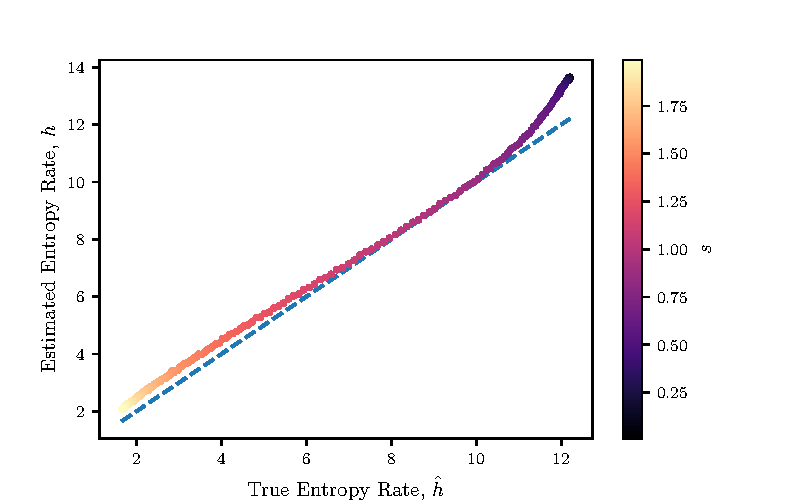
\includegraphics{chapter2/figs/convergence_to_truth.pdf}
\caption{Estimated entropy rates and analytic entropy rates of sequences of 20,000 i.i.d. Zipf distribution random variables with scaling parameter $\alpha$. Dashed line represents the true entropy rate equalling the entropy rate estimate. As values for $\alpha$ approach 0 the high variance of the distributions results in poor estimates due to the finite sample of the Zipf distribution. \label{figs:entropy:convergencetotruth}}
\end{figure}

For values of $\alpha$ between 2 and 0.5, the entropy rate estimate appears to be a rough upper bound on the true entropy rate of the process. This upper bound is only achieved with sufficient lengths of sequences such that the estimator can converge to this upper bound. Indeed, given sufficient length the variance of the estimates on sequences drawn from the same distribution is very low. This is in contrast to the bias of the estimate, which varies with the changing scaling parameter. 

When $\alpha$ becomes lower than 0.5, the Zipf distribution becomes more evenly distributed with reduced skew. This results in a larger probability of low rank word occurrences, producing a process where many words appear very few times. As a result, the finite nature of the sequence results in a entropy rate estimate that grows faster than the true entropy, increasing the bias for these high entropy sequences. 

In general, the convergence of the estimator is sufficient, with a slight caveat: while the estimator convergences to an estimate tightly with very little variance, the bias of the estimate is not constant and varies with the complexity of the sequences. While this finding is itself interesting and warrants future work, the estimator is both consistent and its estimates appear monotonic with the true entropy rate. As such, we will use this estimator to approximate the true entropy rate moving forward, with a cautious eye to the possible effects of this inconsistent bias. 
%</Zipf real entropy>

%<Real data entropy convergence>
To extend from this result, we apply the same approach replacing Zipf distribution generation with text from the news-source Twitter data. 5000 tweets are drawn uniformly from the collection of all tweets from all news-media outlets. These tweets are tokenized and concatenated into a single sequence of natural language text ranging from 85,000 to 90,000 tokens.

Unlike the case of Zipf, we cannot show a true entropy rate for this distribution, as it's unknown, but can demonstrate its convergence.  Each sample has the entropy rate calculated using only the first $N$ tokens, up to the length of 60,000 tokens. \autoref{fig:entropy:realconvergence} shows the clear convergence of the estimator on the real data, approaching an entropy rate of 7.53. As with the Zipf simulations, the variance of the estimated entropy rates of the samples reduces as more tokens are included in the estimate.  The real data takes longer to converge, needing up to 50,000 tokens to achieve a variance of less that $10^{-3}$.

\begin{figure}[!htbp]
\centering
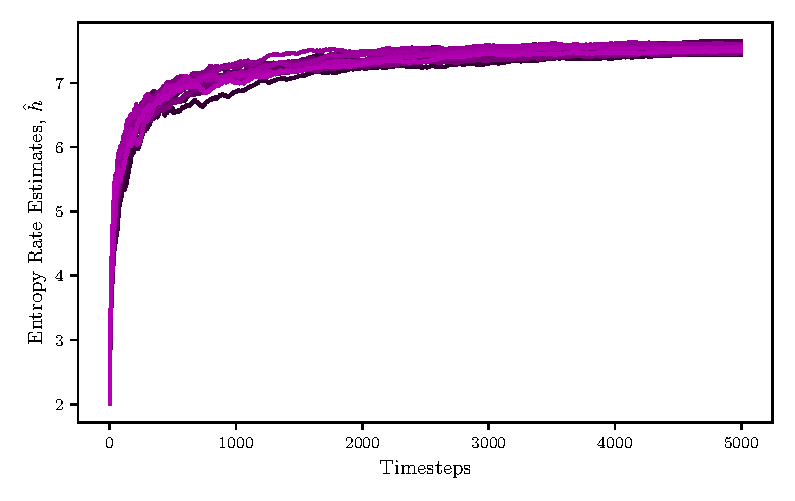
\includegraphics{chapter2/figs/real_entropy_convergence.pdf}
\caption{Convergence of the Kontoyiannis entropy rate estimator on sequences words generated by drawing tweets uniformly without replacement from the pool of all tweets produced by all news-media organisations. Multiple sequences are drawn with most convergence curves overlapping. \label{fig:entropy:realconvergence}}
\end{figure}

%</Real data entropy convergence>

%<Tikz of flow>
\subsubsection{Self entropy rate summary}

\begin{figure}[!htbp]
	\centering
	\includestandalone[width=\textwidth]{chapter2/figs/tikz/self_flow}
	\caption{A conceptual diagram of entropy rate estimation using the Kontoyiannis entropy rate estimation. Tweets shown as blue rectangles are positioned in time and contain textual content. Content proceeding the position \emph{Now} will have snippets of text matched with text from the history of the process, denoted by {\color{orange}orange} and \underline{underlined} text. These text matches are used to calculate $\Lambda_i$ which is used in the entropy estimate. \label{fig:entropy:selfflow}} 
\end{figure}

Before moving away from the entropy rate of a single process, we visualise the how the Kontoyiannis entropy rate estimator works for real data. \autoref{fig:entropy:selfflow} shows a simplified version of the conceptual entropy rate calculation. For a given Twitter user, tweets appear sequentially, separated in time. At any given time, the content of the immediate future of that user's tweets is compared to the entire history of the tweets before that time. This process is then repeated for all possible times in the data. In essence, the calculation of the $\Lambda_i$ is a repeated examination of how much of the immediate complexity at timestep $i$ can be described using the history of the sequence. In total, this estimator provides an average of how many bits are needed to describe the future of this process given its past at any point. 

%% Histogram of self entropy rates ??

%</Tikz of flow>

\section{Cross entropy rate}

To create a notion of information flow, we need to move beyond looking at an individual source in isolation. To do so, we need a tool of comparison between sources rooted in our tools from information theory. We find such a tool in a generalisation to a Kontoyiannis cross entropy rate.

Similar to the extension of entropy, $$H(X) = \sum_{x \in \mathcal{X}} p(x)\log p(x)=-\mathbb{E}[\log P(X)],$$ to cross entropy, $$H(p,q) = \sum_{x \in \mathcal{X}} p(x)\log q(x) = -\mathbb{E}_p[\log q(X)],$$  in \autoref{def:crossentropy}, we can generalise our notion of Kontoyiannis entropy rate from \autoref{def:Kontoyiannis} to a \emph{cross} entropy rate which we will call the Kontoyiannis cross entropy rate. This Kontoyiannis cross entropy rate comes in two forms, a full cross entropy and a time-synced cross entropy.

\begin{definition}[Kontoyiannis Full Cross Entropy Rate]
	The cross entropy rate of a {\color{target} target process} $\mathcal{T}$ coded from a {\color{source} source process} $\mathcal{S}$ can be estimated via,
	\begin{equation}
	H(\mathcal{T} || \mathcal{S})=\frac{N_{\mathcal{T}} \log _{2} N_{\mathcal{S}}}{\sum_{i=1}^{N_{\mathcal{T}}} \Lambda_{i}(\mathcal{T}| \mathcal{S})}
	\end{equation}
	Where $N_{\mathcal{X}}$ is the length of process $\mathcal{X} \in \{\mathcal{T}, \mathcal{S}\}$ and $\Lambda_{i}(\mathcal{T}| \mathcal{S})$ is given by the shortest subsequence starting at position $i$ in the {\color{target}target} $\mathcal{T}$ that does not appear as a contiguous subsequence anywhere in the {\color{source}source} $\mathcal{S}$.
	\begin{equation}
	\Lambda_{i}(\mathcal{T}| \mathcal{S}) = \max \left\{\ell: T_i^{i+\ell}=S_{j}^{j+\ell}, 0 \leq j \leq N_{\mathcal{S}},  0 \leq \ell \leq \min( N_{\mathcal{S}}- j , N_{\mathcal{T}}- i )\right\},
	\end{equation}
	where $T_a^{b}$ and $S_a^b$ are continuous subsequences starting from index $a$ to index $b$ of the {\color{target} target}, $\mathcal{T}$, and  {\color{source} source}, $\mathcal{S}$, processes respectively.
\end{definition}

This approach to cross entropy matches segments of text in the {\color{target}target} to segments of text anywhere in the {\color{source}source} in the same manner that the Kontoyiannis entropy rate matched segments of text in the future of a process from a index, $i$, to the history before the index. In contrast to the entropy rate estimate, which asked how much information was needed on average to \emph{describe the future of a source from its past}, this cross entropy rate estimate is asking how much information is needed on average to \emph{describe the target given full knowledge of the source}. 

\begin{figure}[!htbp]
	\centering
	\includestandalone[width=\textwidth]{chapter2/figs/tikz/unsynced_flow}
	\caption{A conceptual diagram of Kontoyiannis full cross entropy rate estimation. Tweets shown as rectangles are positioned in time for both a target and source, containing textual information. Content in the {\color{source}source} is matched with content in the immediate future of the {\color{target}target} for a given time point, $t$, to calculate match-lengths. This time point is shifted along the {\color{target}target} timeline to average match-lengths and calculate the full cross entropy rate.\label{fig:entropy:unsyncedflow}} 
\end{figure}

This full knowledge over all of the process gives the estimator the `Full' in its title, but presents a impropriety. In the context of our problem, this estimator is cheating by viewing the future of news through the lens of the source process. 

As \autoref{fig:entropy:unsyncedflow} illustrates, the text subsequence match in the target could be drawn from future time points in the source. Restated, the cross entropy rate will, in-part, be describing how much information is needed to encode the future of a piece of target news already knowing the future of the news from another source. While this may be an interesting insight in itself, and could be used in future work to format a notion of information divergence, it doesn't probe the underlying process of \emph{information flow} with which this thesis focuses. 

Rather than looking at the entire lifetime of the source during the matching calculations, we can reduce our search space to the text that occurred in the \emph{past} of the source. To achieve this we use an important piece of our data, the time that tweets occurred. For each word in the target process, $T_i$ has an associated time with it, $t(T_i)$. When matching the future of $\mathcal{T}$, starting from an index $i$, we can reduce the source process, $\mathcal{S}$ to only the words that were themselves tweeted before time $t(T_i)$. 

Put simply, we can alter the Kontoyiannis full cross entropy rate to a time-synced cross entropy rate by replacing the full source process, $\mathcal{S}$, with a time reduced source process $\mathcal{S}_{ \leq t(T_i)}$. This can be seen visually in \autoref{fig:entropy:timesyncedflow} and is formally defined as follows.

\begin{definition}[Kontoyiannis Time-synced Cross Entropy Rate]
	The time-synced cross entropy rate of a {\color{target}target} process $\mathcal{T}$ coded from a {\color{source}source} process $\mathcal{S}$ can be estimated via,
	\begin{equation}
	H(\mathcal{T} || \mathcal{S})=\frac{N_{\mathcal{T}} \log _{2} N_{\mathcal{S}}}{\sum_{i=1}^{N_{\mathcal{T}}} \Lambda_{i}(\mathcal{T}| \mathcal{S}_{\leq t(T_i) } )}
	\end{equation}
	Where $\Lambda_{i}(\mathcal{T}| \mathcal{S}_{\leq t(T_i) })$ is given by the shortest subsequence starting at position $i$ in {\color{target}target} $\mathcal{T}$ that does not appear as a contiguous subsequence in the time reduced {\color{source}source} $\mathcal{S}_{\leq t(T_i) }$ where,
	\begin{equation}
	\mathcal{S}_{\leq t(T_i) } = \{S_j | t(S_j) \leq t(T_i),  \forall i \}.
	\end{equation}
	Which gives,
	\begin{align*}
	\Lambda_{i}(\mathcal{T}| \mathcal{S}_{\leq t(T_i)}) = \max \{\ell: T_i^{i+\ell}=S_{j}^{j+\ell}, 0 \leq j \leq N_{\mathcal{S}},  \\  0 \leq \ell \leq \min( N_{\mathcal{S}}- j , N_{\mathcal{T}}- i ) \},
	\end{align*}
	where $T_a^{b}$ and $S_a^b$ are continuous subsequences starting from index $a$ to index $b$ of the {\color{target} target}, $\mathcal{T}$ process, and the time reduced {\color{source} source}, $\mathcal{S}_{\leq t(T_i)}$, respectively.
\end{definition}

\begin{figure}[!htbp]
	\centering
	\includestandalone[width=\textwidth]{chapter2/figs/tikz/timesynced_flow}
	\caption{A conceptual diagram of Kontoyiannis time-synced cross entropy rate estimation. Tweets shown as rectangles are positioned in time for both a target and source, containing textual information. Content in the {\color{source}source} that occurs before time $t$ is matched with content in the immediate future of the {\color{target}target} from $t$ to calculate match-lengths. This time point is shifted along the {\color{target}target} timeline to average match-lengths and calculate the time-synced cross entropy rate.\label{fig:entropy:timesyncedflow}} 
\end{figure}


% Informantion flow idea
This time-synced cross entropy rate is testing not just the differences in the language processes of the source and target, but also measuring what information in the target is present in the source's history. This is an important distinction, as it allows us to probe a very important aspect of our data, namely, the time in which news is created. 

If a piece of information appears earlier in the source than in the target, it will be detected during the match length search, resulting in a lower entropy. This is to say, in the context of news, if the {\color{source}source} breaks a story first, \emph{less} information is required to describe the subsequent news output from the {\color{target}target}. 

Conversely, if a {\color{target}target} produces a piece of information before the {\color{source}source}, then that information will not appear in the history of the time-synced source during the match-length search. This will result in lower values of $\Lambda_i$ for that piece of information, which raises the cross entropy rate.

From this, we can find that, on average, if a {\color{source}source} produces information earlier than a {\color{target}target}, the cross entropy rate, $\hat{h}(\mathcal{T} || \mathcal{S})$, will be lower than if the {\color{target}target} produces information earlier than the {\color{source}source}. This method of examining who produces information first can be extended into a notion of \emph{information flow}, a discussion we will leave for \autoref{ch:quotermodel}.


\subsection{Validating the assumptions of cross entropy estimation}

To validate these new cross entropy rate estimators a similar process is performed as with the entropy rate. Fortunately, many of the assumptions transfer over directly.

In the case of ergodicity, stationarity and the Doeblin Condition, all three are properties of the process under investigation, which we argued above are well founded. We introduce an additional condition on the processes for the sake of cross entropy rates, namely that the processes have the same state space. This additional condition extends the earlier conditions to apply jointly between both the source and target processes. While not all news-media organisations will have the same realisations of words in their corpus, the processes could be reasonably thought to have the same state space, as all processes are using English and discussing similar topics.

This then leads naturally to the next question of convergence. Following a similar process of uniform withdrawals from a distribution will result in functionally similar convergence to the entropy rate above. Indeed, this can be seen in \autoref{fig:entropy:realcrossconvergence}, where tweets are draw uniformly from the pool of all tweets and cross entropy rates are calculated on the resulting sequences. Here, the cross entropy rate is denoted $\hat{h}_{\times}$ to distinguish from the entropy rate estimates $\hat{h}$. This figure is, as expected, functionally similar to \autoref{fig:entropy:realconvergence} from the entropy rate section above. This cross entropy rate calculation is fundamentally no different from the original entropy rate calculation with these sequences, as a randomly selected history of another process is just a useful and a randomly selected history the original process when both draw from the same distribution.


\begin{figure}[!htbp]
	\centering
	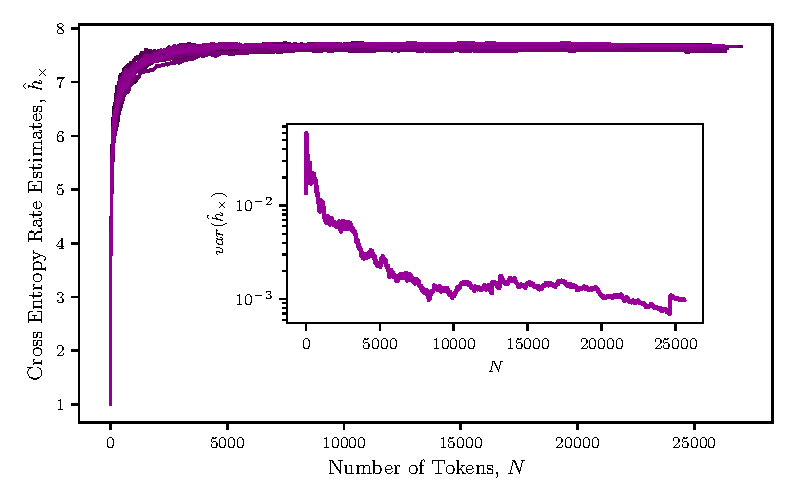
\includegraphics{chapter2/figs/cross_real_entropy_convergence}
	\caption{Convergence of the Kontoyiannis time-synced cross entropy rate estimator on pairs of sequences independently generated by drawing tweets uniformly without replacement from the pool of all tweets produced by all news-media organisations.} \label{fig:entropy:realcrossconvergence}
\end{figure}

A more nuanced investigation of the cross entropy convergence emerges when we utilise processes with \emph{different} distributions. \autoref{fig:entropy:zipfcrossconvergence} does exactly this. Using pairs of scaling parameters for different Zipf distributions, simulations of 30,000 long i.i.d.~ processes are made with separate target and source processes. The cross entropies rates are then estimated across these pairs. When the scaling parameters are equal, $\alpha_{source}=\alpha_{target}$, we observe the same entropy and convergence pattern as we would for a single i.i.d. process with that distribution. 

\begin{figure}[!htbp]
	\centering
	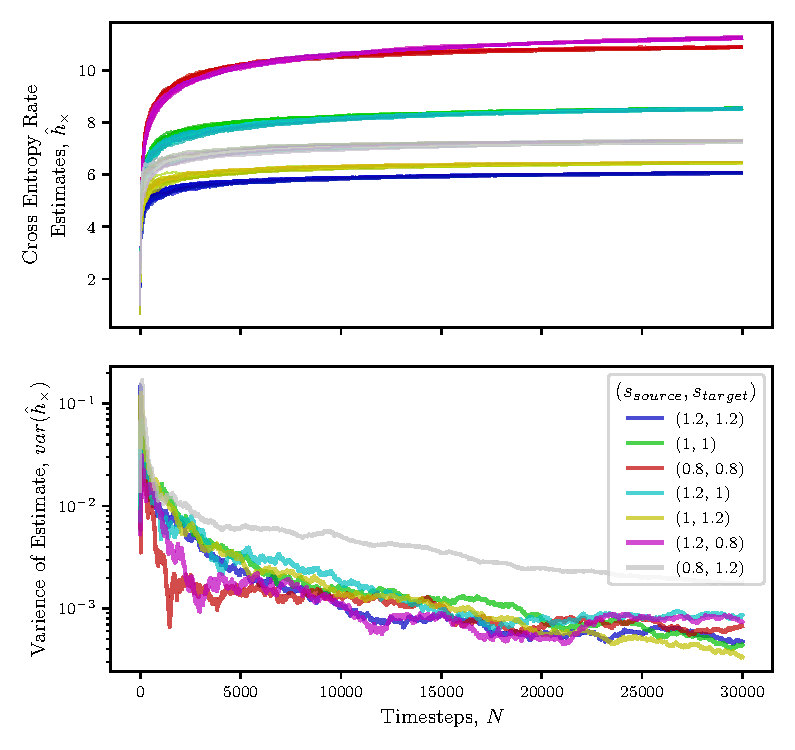
\includegraphics{chapter2/figs/cross_Zipf_entropy_convergence.pdf}
	\caption{Convergence of the Kontoyiannis time-synced cross entropy rate estimator on pairs sequences of i.i.d. Zipf distribution realisations with varying pairs of Zipf distribution rates, $\alpha_{source}$ and $\alpha_{target}$. } \label{fig:entropy:zipfcrossconvergence}
\end{figure}

When $\alpha_{source} \neq \alpha_{target}$ the entropy rates vary, and are not always similar to the entropy rate of the target or the source. Most cross entropy rates converge at a similar pace to the entropy rates above, although large deviations between distributions can reduce this rate of convergence. In particular when the source has significantly higher complexity than the target, as in the case of $(\alpha_{source}, \alpha_{target}) = (0.8,1.2)$, the entropy takes much longer to converge as it requires longer for common patterns to occur in the high complexity source for sequence matching. % talk more





\subsection{Predictability}
With the Kontoyiannis cross entropy rate estimator converging, we also want to generalise the notion of maximal predictability.
We introduced maximal predictability, $\pi^{max}(S,V)$,  in \autoref{def:maximialpredictability} as it is a robust way of determining an upper bound on how well the future of a process could be predicted from its past. The use of the state space size, allows for normalisation of the entropy rate when state spaces are large. The state space size will be represented as $V$ as the state space of language is the vocabulary.

In order to generalise this notion of maximal predictability, we need to identify the two replacements for the inputs. The replacement for entropy rate is trivially the cross entropy rate, but the choice of state space size is more nuanced. Three choices are possible, the state space of the source, $V_{source}$, the target, $V_{target}$, and the union of the state spaces $V_{union}$. 

The original motivation behind the maximal predictability is to normalised the entropy by \emph{how complex the system we are trying to predict is}. This complexity is a property of the target. While a complex source does change how well the target can be predicted, it is the property of the target that needs to be controlled for. As such, the choice of $V_{target}$ is taken and referred to as simply $V$ in the following definition.

\begin{definition}[Maximal Cross Predictability]
For two processes $S$ and $T$ with cross entropy $H(T||S)$ from the source to the target and state space size $V$ of the target, the maximal cross predictability, $\pi^{max}(T||S)$ can be found numerically by solving, 
\begin{equation}
H(T||S)  = H(\pi^{max}(T||S)) + (1 - \pi^{max}(T||S)) \log (V - 1),
\end{equation}
for $\pi^{max}(T||S)$.
\end{definition}


\subsection{A note on package development}

As stated earlier, a key challenge in estimating these Kontoyiannis cross entropy rates is calculation speed. With time complexities of $O(N^3)$ on the number of input tokens, efficient code is necessary to allow for estimation using long sequences. To achieve speed and contribute to this field of work more broadly, a speed-focused open source package was developed to help researchers efficiently and easily calculate entropy rates such as those discussed above. The important snippets from code contributions of the package, named `ProcessEntropy', are available in \autoref{app:code} and this section will outline tools used in speeding the code up.

Fundamental complexity limitations of the subsequence matching algorithm mean that speed improvements need to come from smart implementation. Two techniques used are interesting enough to discuss briefly here, hashing and just-in-time compilation.

In the context of analysing language like a process, each word is simply an element of the state space. As such, each word can be assigned a unique number to represent its position in the state space. In doing so it allows the computations of the $\Lambda_i$'s to be performed using much faster integer operations. In the ProcessEntropy package, words are converted to 32 bit unsigned integers using Fowler–Noll–Vo hashing. Fowler–Noll–Vo is a non-cryptographic hash function which is fast to compute. This converts words to the same integer every time, with no collisions. 


The second major speed improvement is drawn from the use of just-in-time (JIT) compilation. Python is commonly used in scientific settings as an interpreted language. In most contexts the Python interpreter allows variables to exist as dynamic types. As such, the exact same function can often be applied to integers, strings or other objects interchangeably. As a result, a larger number of type checks and other control operations are required during runtime, slowing down computation. JIT compilers such as Numba\footnote{\url{https://numba.pydata.org/}} operate by observing variable types at the start of runtime and generating optimized machine code. 

\begin{figure}[!htbp]
\centering
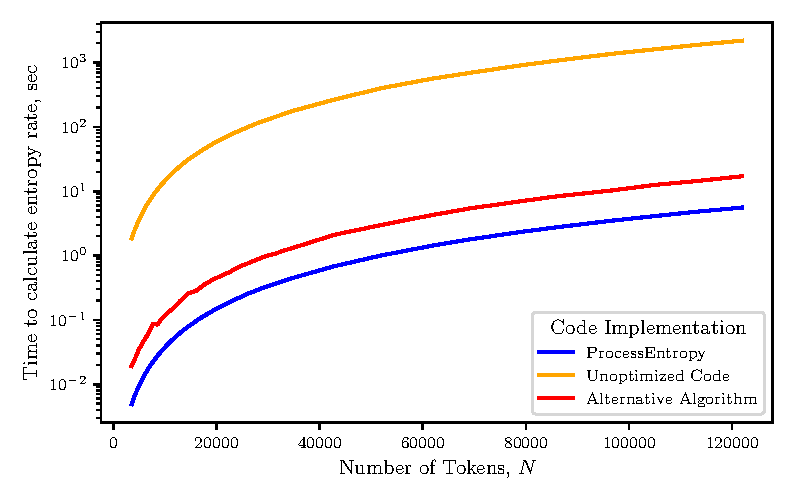
\includegraphics{chapter2/figs/speedcomparison.pdf}
\caption{A speed comparison of implementations of the Kontoyiannis entropy rate estimator. ProcessEntropy uses code from the package of the same name, unoptimized code is the same algorithm as ProcessEntropy without type and compile optimizations and Alternative Algorithm is an optimized alternative algorithm using the built-in \texttt{.contains()} method from the \texttt{stringlib} library. \label{fig:entropy:speedcomparison}}
\end{figure}


\autoref{fig:entropy:speedcomparison} shows a comparison of the optimized methods compared to alternatives. The ProcessEntropy package consistently performs the fastest, using the speed improvements listed above and efficient implementation. In contrast, the unoptimized code (written in pure Python without fixed type compiling or parallelisation) performs over two orders of magnitude slower for all input sizes. For comparison, an alternative algorithm is shown using the highly optimized \texttt{.contains()} method included in the \texttt{stringlib} library from Cython. This method uses a simplified version of the Boyer-Moore string-search algorithm, incorporating ideas from Horspool and Sunday~\cite{lundh_stringlib_2006}. Even with the alternative algorithm written in C, the ProcessEntropy code outperforms consistently. The package is available on the Python Package Index (PyPi) for interested researchers\footnote{\url{https://pypi.org/project/ProcessEntropy/}}.

\subsection{Running estimations}\label{sec:running_estimations}

To close this chapter, the tools developed throughout can now be applied to the news dataset introduced in \autoref{ch:data}. This news data contains 154 year-long Twitter content streams, with mean of 337,284 tokens. %
%(min 8059, max 2,627,305, $\sigma=$377,994)
Each stream has its entropy rate calculated and each pair of news-media outlets have their time-synced cross entropy rate calculated in both directions. In total this is 23,716 entropy rate estimations on these long sources. Even, with the efficient ProcessEntropy package, these calculations take well over a week, and this analysis would not be computationally tractable on the available hardware using the other implementations of the code.


\begin{figure}[!htbp]
	\centering
	\begin{subfigure}[t]{0.58\textwidth}
		\centering
		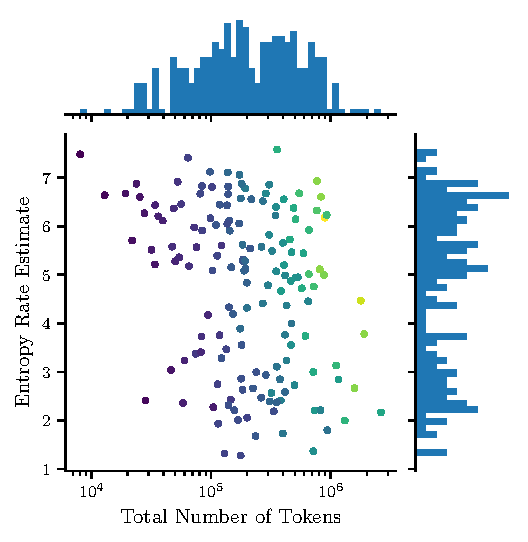
\includegraphics{chapter2/figs/tokens_vs_self_entropy_rate.pdf}
		\caption{}
	\end{subfigure}
	~
	\begin{subfigure}[t]{0.38\textwidth}
		\centering
		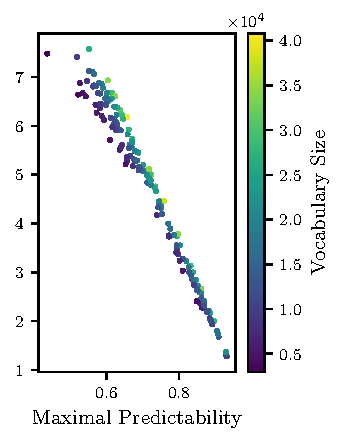
\includegraphics{chapter2/figs/entropy_vs_predictability.pdf}
		\caption{}
	\end{subfigure}
	\caption{Entropy rate estimates for the Twitter timelines of 154 news-media organisations during the calendar year of 2019. (a) shows the limited relationship between the total number of tokens in the Twitter text history and the entropy rate estimates. (b) shows the tight relationship between the entropy rates estimate and its derived maximal predictability, with higher variances seen at high entropies.}
	\label{fig:entropy:selfentropyrateestimates}
\end{figure}

\autoref{fig:entropy:selfentropyrateestimates} shows these entropy rate estimates on the news-media Twitter histories. Importantly, the entropy rate estimate shows very limited correlation with the total length of the content (number of tokens) or with the vocabulary size. This indicates that the estimate entropy rates have converged. Further, we see an expected strong correlation between the entropy rate estimate and the maximal predictability. Notably, the variance between the two increases for higher entropy rates, where larger vocabulary sizes can have an outsized effects on estimates. 

\begin{figure}[!htbp]
\centering
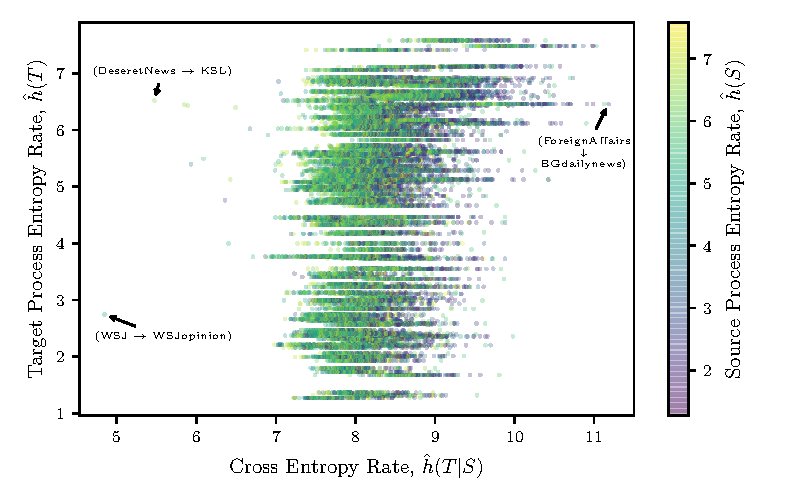
\includegraphics{chapter2/figs/cross_vs_self_entropy_rates.pdf}
\caption{Time-synced cross entropy rate estimates on pairs of news-media organisations on Twitter using their full content for the 2019 calendar year. Cross entropy rates are compared to the entropy rate estimates of the sources, $S$, and targets, $T$, in isolation. Example outliers are shown as `(source $\to$ target)'.} \label{fig:entropy:crossentropyestimates}
\end{figure}

Following this, the time-synced cross entropy rates are estimated and shown in \autoref{fig:entropy:crossentropyestimates}. Here we see similar results. The target entropy rate has limited correlation with the cross entropy rate ($R^2=0.116$), except for very high entropy targets, which receive higher cross entropy rates due to the high complexity nature of the target information. In contrast, source entropy rate has almost no correlation with the cross entropy rate ($R^2=0.0497$).

Several outliers exist at both the high and low ends of cross entropy. Low cross entropy outliers are all pairs of news-media organisations which are deeply related. Two examples of this are (\emph{@WSJ} $\to$ \emph{@WSJopinion}), where the information in the \emph{Wall Street Journal's} Opinion news stream can be described extremely efficiently by the \emph{Wall Street Journal's} main news stream, and (\emph{@DeseretNews} $\to$ \emph{@KSL}), where both news-media organisations report news specifically about Salt Lake City, Utah, and \emph{Deseret News} previously owned and remains closely linked to \emph{KSL}. 

At the high end of the cross entropy, pairs of organisations tend to have very little relationship. The highest cross entropy rate pair is (\emph{@ForeignAffairs} $\to$ \emph{@BGdailynews}) which suggests that very little information from the international relations focused \emph{Foreign Affairs Magazine} is useful in describing `Southcentral Kentucky's No. 1 Source for Information' \emph{Bowling Green Daily News}.

In total, the cross entropy rates are much higher than the entropy rates, highlighted in \autoref{fig:entropy:estimatedesnities}. This is an expected behaviour, as predicting the language and content behaviour of someone else is naturally harder than predicting your own future text. These distributional differences are carried over into maximal predictability, with generally lower maximal cross predictabilities.

\begin{figure}[!htbp]
	\centering
	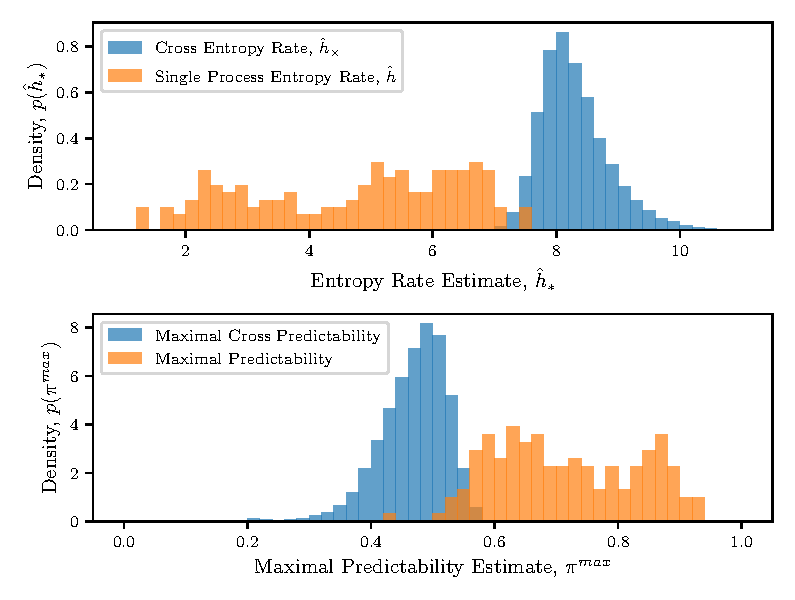
\includegraphics{chapter2/figs/entropy_densities.pdf}
	\caption{Comparison of cross and individual measures of information complexity. Self entropy rates and self maximal predictabilities are calculated for each of the 154 news-media organisations. Cross entropy rates and cross maximal predictabilities are calculated for all pairs of organisations. The distribution of the cross information and self information estimates are compared.
	Cross entropy rates are higher than self entropy rates as news-media organisations, in general, do not contain information in their history that is more useful to other news-media organisations than it is to themselves. This is reflected in the lower maximal cross predictabilities.  } \label{fig:entropy:estimatedesnities}
\end{figure}

\subsubsection{Concluding remarks}
Using both the Kontoyiannis entropy rate estimate and the generalised Kontoyiannis cross entropy rate estimate, we can construct a set of summary statistics about the language and behaviour patterns of the news sources under investigation and their relationships. These estimators are well founded on both a theoretical backbone and experimental evidence, and can be applied efficiently using the new open-source package, ProcessEntropy. From here, these calculated estimates can be used to extract the measures of information flow sought in this thesis, a task for \autoref{ch:quotermodel}.




%!TEX root = ../thesis.tex
\chapter{Introduction \label{ch:intro}}



The main source of data for analysis is draw from the Twitter accounts of news-media organisations. In the 1950s, the widespread popularity of household television allowed TV broadcasting to become the primary tool for influencing public opinion in developed nations~\todo{cite: Diggs-Brown, Barbara (2011) Strategic Public Relations: Audience Focused Practice p.48}.  This was a shift from a population that \emph{listened} to radio news, to a population that \emph{watched} news. 

The even more rapid rise of mobile internet and social media sites in the last two decades has caused another shift. No longer just a population that watch news at fixed time, or read regularly scheduled newspapers; the conveniences of the modern developed world allow individuals to consume news anytime, anywhere. As of 2019, 55\% of US adults get their news from social media either `often' or `sometimes'~ and 88\% state that `social media companies have at least some control over the mix of news people see'~'\cite{shearerAmericansAreWary2019}.

Given the importance of a free press and the role of social media sites in the delivery of news, this work aims to study the news on social media. To begin this task, we first define some common terms for clarity.

\begin{definition}[Social media]
	The platforms used to consume information by individuals in the public. E.g. Twitter, Facebook, Reddit.
\end{definition}

\begin{definition}[News-media]
	The organisations that are producing information about a broad range of current events and sharing that information with the public.
\end{definition}

\begin{definition}[News]
	The \emph{content} produced by news-media organisations. 
\end{definition}

\section{Data}

Using the media analysis source AllSides\footnote{www.allsides.com}, a collection of news-media organisations was found. The purpose of AllSides is to provide a public analysis of political leanings of news sources~\todo{cite: https://www.allsides.com/media-bias/media-bias-ratings}, and to aggregate news allowing consumers to view articles from different sides of the political spectrum. Each news source is labelled into one of 5 categories, Left, Lean Left, Center, Lean Right, or Right. Any news source the ratings are determined internally using `blind surveys of people across the political spectrum, multi-partisan analysis, editorial reviews, third party data, and tens of thousands of user feedback ratings'~\todo{cite: same as above}. News sources are only assigned to a single category, but do have an attached confidence rating.

From the website, a list of possible news sources was collected on February 1st, 2019. In this collection was organisation names, political bias', the number of user feedback ratings of the political bias, and, if available, the twitter handles associated with those sources. These collected news sources were broad, containing not just news-media organisations but authors, pundits and think tanks. 

To select an appropriate set of news-media organisation an examination and filtering process was undertaken. A source was only considered if it was a organisation (not an individual), that produced news content of a diverse range of topics. Many news sources were connected to think tanks or opinion groups, and only created news of a single topic or campaign. Further, if an news-media organisation has no twitter account or had less than 10,000 followers (a low bar in the social media world), then it was removed from the pool. This mainly removed inactive organisation and news organisation from small rural towns. Finally, a single sources was removed as it was not in English, and a single source was removed as it was the smaller sister site that had all content as a subset of it's larger site.  The result of this filtering process is 174 news-media organisations and associated twitter accounts and categorised political bias'.  A list of all news-media organisations under analysis can be seen in \todo{appendix of success} and all removed sources and the removal justification can be seen in \todo{appendix of removals}.

%twitter collection






% add as many as you like

\appendix
% Import the appendices 
%%!TEX root = ../thesis.tex
\chapter{News Media Twitter Accounts\label{app:accounts}}

\subsection{Included Organisations}

\begin{table}[h]
	\caption{\todo{Caption}}
	\label{appendix:tab:accounts_0}
	\begin{center}
		\resizebox{1 \textwidth}{!}{\begin{tabular}{lllrr}
\toprule
                    Name &  Twitter Account & Assigned Bias &  Number of Tweets &  Followers \\
\midrule
      The New York Times &          nytimes &     Lean Left &             31029 &   44800317 \\
                     CNN &              cnn &          Left &             57155 &   44153462 \\
        BBC News (World) &         BBCWorld &        Center &             11679 &   26446876 \\
           The Economist &     theeconomist &     Lean Left &             35771 &   24239639 \\
                 Reuters &          reuters &        Center &            128448 &   21042215 \\
 The Wall Street Journal &              WSJ &        Center &             32151 &   17139922 \\
                    TIME &             time &     Lean Left &             29631 &   16512854 \\
                  Forbes &           Forbes &        Center &             31940 &   15736852 \\
                ABC News &              ABC &     Lean Left &             44149 &   14804638 \\
     The Washington Post &   washingtonpost &     Lean Left &             45043 &   14644580 \\
    The Associated Press &               ap &        Center &             10214 &   13671750 \\
                HuffPost &         huffpost &          Left &             27622 &   11472382 \\
              TechCrunch &       techcrunch &        Center &             14348 &   10124437 \\
                Mashable &         mashable &          Left &             40854 &    9809420 \\
          The New Yorker &        newyorker &          Left &             13948 &    8774527 \\
          The Daily Show &     thedailyshow &     Lean Left &              3386 &    8256511 \\
            The Guardian &         guardian &     Lean Left &             77532 &    8243012 \\
                     NPR &              npr &        Center &             21236 &    7959364 \\
                CBS News &          CBSNews &     Lean Left &             34060 &    7078950 \\
           Rolling Stone &     RollingStone &          Left &             18571 &    6295950 \\
               Bloomberg &         business &        Center &            109367 &    5790419 \\
             VANITY FAIR &       vanityfair &     Lean Left &             15585 &    4887894 \\
                   TODAY &        TODAYshow &     Lean Left &             17678 &    4282063 \\
              Lifehacker &       lifehacker &        Center &              9026 &    4153410 \\
                POLITICO &         politico &     Lean Left &             25742 &    4016243 \\
               USA TODAY &         usatoday &        Center &             27303 &    3949159 \\
         Financial Times &               FT &        Center &             41030 &    3806483 \\
     Scientific American &            sciam &        Center &              2335 &    3805593 \\
                The Hill &          thehill &        Center &            157172 &    3501890 \\
       Los Angeles Times &          latimes &     Lean Left &             35341 &    3473994 \\
                Newsweek &         newsweek &     Lean Left &             46922 &    3407905 \\
              Teen Vogue &        TeenVogue &     Lean Left &             12270 &    3358001 \\
                    CNBC &             cnbc &        Center &             66578 &    3355408 \\
                   MSNBC &            msnbc &          Left &             32699 &    2870702 \\
        Business Insider &  businessinsider &        Center &             57915 &    2790009 \\
           The Telegraph &        Telegraph &    Lean Right &             24235 &    2774439 \\
               The Verge &            verge &     Lean Left &             19096 &    2613577 \\
       Daily Mail Online &       MailOnline &         Right &             28671 &    2437611 \\
                    VICE &             vice &          Left &             17195 &    2000034 \\
                   CSPAN &            cspan &        Center &              5022 &    1989017 \\
\bottomrule
\end{tabular}
}
	\end{center}
\end{table}

\begin{table}[h]
	\caption{\todo{Caption}}
	\label{appendix:tab:accounts_1}
\begin{center}
\resizebox{1 \textwidth}{!}{\begin{tabular}{lllrr}
\toprule
                   Name & Twitter Account & Assigned Bias &  Number of Tweets &  Followers \\
\midrule
           The Atlantic &     theatlantic &     Lean Left &             15100 &    1850164 \\
      New York Magazine &           NYMag &          Left &             19072 &    1800255 \\
                  Slate &           slate &          Left &             58598 &    1792093 \\
        Al Jazeera News &         AJENews &        Center &             11252 &    1573047 \\
          New York Post &          nypost &         Right &             79771 &    1543609 \\
          BuzzFeed News &    BuzzFeedNews &     Lean Left &             19705 &    1338555 \\
         Breitbart News &   BreitbartNews &         Right &             17501 &    1225203 \\
             Yahoo News &       YahooNews &          Left &             19781 &    1106092 \\
        Chicago Tribune &  chicagotribune &        Center &             22994 &    1099101 \\
                    AJC &             ajc &     Lean Left &             27978 &    1045546 \\
           PBS NewsHour &        NewsHour &        Center &             16189 &    1036993 \\
                  Salon &           salon &          Left &             11614 &     976078 \\
                    Vox &       voxdotcom &          Left &             17574 &     891290 \\
             ProPublica &      propublica &        Center &              6458 &     833038 \\
           Mother Jones &     motherjones &          Left &             16447 &     809121 \\
       The Boston Globe &     bostonglobe &     Lean Left &             49224 &     756522 \\
          The Intercept &    theintercept &          Left &              6642 &     753001 \\
    New York Daily News &     nydailynews &          Left &             28682 &     728512 \\
        Foreign Affairs &  ForeignAffairs &        Center &             11964 &     724994 \\
 New York Times Opinion &      nytopinion &          Left &             25402 &     718663 \\
         Democracy Now! &    democracynow &          Left &              9453 &     710714 \\
               TheBlaze &        theblaze &         Right &             13121 &     706991 \\
           Daily Caller &     DailyCaller &         Right &             34716 &     579741 \\
               The Root &         TheRoot &     Lean Left &              6994 &     525879 \\
               Upworthy &        upworthy &          Left &              1472 &     511090 \\
       One America News &            OANN &    Lean Right &              6108 &     510392 \\
      Chicago Sun-Times &        Suntimes &     Lean Left &             15976 &     505161 \\
                 SFGate &          sfgate &     Lean Left &             17838 &     477782 \\
           Miami Herald &     MiamiHerald &     Lean Left &             19290 &     450869 \\
     The Jerusalem Post &  Jerusalem\_Post &        Center &             29868 &     445004 \\
                Esquire &         esquire &          Left &             12817 &     418881 \\
                 Quartz &              qz &        Center &             28604 &     384220 \\
   The Washington Times &       WashTimes &    Lean Right &             34635 &     372421 \\
              Roll Call &        rollcall &        Center &             10157 &     361580 \\
         The Daily Wire &   realdailywire &         Right &             26385 &     361505 \\
        National Review &             NRO &         Right &             16572 &     336300 \\
                  Axios &           axios &        Center &             19184 &     315533 \\
       Austin Statesman &       statesman &     Lean Left &              9562 &     300429 \\
              Daily Kos &        dailykos &          Left &             12636 &     280636 \\
                 reason &          reason &    Lean Right &              7939 &     242262 \\
\bottomrule
\end{tabular}
}
\end{center}
\end{table}

\begin{table}[h]
	\caption{\todo{Caption}}
	\label{appendix:tab:accounts_2}
	\begin{center}
		\resizebox{1 \textwidth}{!}{\begin{tabular}{lllrr}
\toprule
                    Name &  Twitter Account & Assigned Bias &  Number of Tweets &  Followers \\
\midrule
            Mercury News &         mercnews &     Lean Left &             36535 &     241228 \\
                 Jacobin &       jacobinmag &          Left &              8579 &     241092 \\
            ScienceDaily &     sciencedaily &        Center &              1243 &     240013 \\
           Las Vegas Sun &      LasVegasSun &     Lean Left &              8233 &     238797 \\
                   grist &            grist &     Lean Left &              6438 &     230344 \\
      The Sacramento Bee &      sacbee\_news &     Lean Left &             22511 &     219066 \\
                RedState &         redstate &         Right &             19778 &     218545 \\
          The Federalist &           FDRLST &         Right &              5830 &     217053 \\
           O.C. Register &       ocregister &    Lean Right &             23872 &     212517 \\
               SF Weekly &         sfweekly &        Center &              4438 &     210524 \\
               Raw Story &         rawstory &          Left &             29702 &     205992 \\
     Washington Examiner &       dcexaminer &    Lean Right &             61833 &     198229 \\
                OBSERVER &         observer &        Center &              5856 &     195067 \\
 San Francisco Chronicle &      sfchronicle &          Left &             18021 &     189685 \\
                     KSL &           KSLcom &         Right &             11881 &     179424 \\
                Truthout &         truthout &     Lean Left &              7806 &     170572 \\
        The New Republic &      newrepublic &          Left &             10725 &     167916 \\
           Investors.com &     IBDinvestors &    Lean Right &              2469 &     167242 \\
 Pittsburgh Post-Gazette &     PittsburghPG &    Lean Right &             24711 &     166684 \\
       Commercial Appeal &      memphisnews &     Lean Left &             15885 &     162002 \\
                Mediaite &         Mediaite &     Lean Left &             14030 &     159980 \\
            Townhall.com &      townhallcom &         Right &             10452 &     152082 \\
               U.S. News &           usnews &     Lean Left &             12827 &     150674 \\
                AlterNet &         alternet &          Left &              7156 &     139194 \\
        National Journal &  nationaljournal &        Center &              1424 &     133097 \\
                The Week &          theweek &        Center &              9031 &     129703 \\
                CBN News &          CBNNews &         Right &             15627 &     128487 \\
    Intl. Business Times &          IBTimes &        Center &             11519 &     123358 \\
             CNSNews.com &          cnsnews &         Right &              9035 &     119236 \\
          Times-Dispatch &          RTDNEWS &    Lean Right &              7018 &     116510 \\
             Free Beacon &       FreeBeacon &         Right &              9091 &     110634 \\
           Boston Herald &     bostonherald &    Lean Right &             12550 &     105046 \\
                 Newsmax &          newsmax &         Right &              3825 &     100437 \\
         Current Affairs &       curaffairs &          Left &              2188 &      99136 \\
            Deseret News &      DeseretNews &    Lean Right &             15087 &      97060 \\
      WSJ Editorial Page &       WSJopinion &    Lean Right &              4990 &      96734 \\
                  Bustle &           bustle &     Lean Left &              1504 &      96170 \\
         Courier Journal &   courierjournal &     Lean Left &             13988 &      88551 \\
   Portland Press Herald &      PressHerald &        Center &              6372 &      85834 \\
             Defense One &       DefenseOne &        Center &              6892 &      81992 \\
\bottomrule
\end{tabular}
}
	\end{center}
\end{table}

\begin{table}[h]
	\caption{\todo{Caption}}
	\label{appendix:tab:accounts_3}
	\begin{center}
		\resizebox{1 \textwidth}{!}{\begin{tabular}{lllrr}
\toprule
                                     Name &  Twitter Account & Assigned Bias &  Number of Tweets &  Followers \\
\midrule
                               The Nation &       The\_Nation &          Left &             13048 &      78860 \\
            The Christian Science Monitor &        csmonitor &        Center &              5676 &      75406 \\
                      AR Democrat-Gazette &   ArkansasOnline &          Left &             10951 &      74177 \\
                                INDY Week &         indyweek &     Lean Left &              4175 &      73802 \\
                             PoliticusUSA &     PoliticusUSA &          Left &              7253 &      72856 \\
                         The Daily Signal &      Dailysignal &         Right &              6740 &      68024 \\
                                 PJ Media &      PJMedia\_com &    Lean Right &              5666 &      66324 \\
                              Delco Times &       delcotimes &     Lean Left &              3302 &      64714 \\
                              Daily Press &      Daily\_Press &    Lean Right &              3512 &      61225 \\
                            YES! Magazine &      yesmagazine &          Left &              4679 &      60455 \\
                          SpokesmanReview &  SpokesmanReview &     Lean Left &              4113 &      58352 \\
                     Tallahassee Democrat &         TDOnline &          Left &             15098 &      53700 \\
                         The Korea Herald &   TheKoreaHerald &        Center &              8730 &      53517 \\
                       The Michigan Daily &    michigandaily &     Lean Left &              2041 &      50748 \\
                      Honolulu Civil Beat &        CivilBeat &        Center &              1837 &      50503 \\
                     Libertarian Republic &   TheLibRepublic &    Lean Right &              1145 &      47475 \\
                The American Conservative &         amconmag &    Lean Right &             25197 &      46189 \\
                   The American Spectator &      amspectator &         Right &              1915 &      45877 \\
                          The Red \& Black &      redandblack &        Center &              7663 &      42735 \\
                                KQED News &         kqednews &        Center &              8655 &      41720 \\
                    Indiana Daily Student &          idsnews &        Center &              3867 &      41621 \\
                                     WGBH &             wgbh &        Center &              2211 &      39971 \\
                      The Western Journal &   WestJournalism &         Right &              7114 &      38478 \\
                      Commentary Magazine &       Commentary &         Right &              1337 &      35704 \\
                       The Daily Progress &    DailyProgress &        Center &              6856 &      35506 \\
                                 VTDigger &         vtdigger &     Lean Left &              5671 &      32820 \\
                            BG Daily News &      bgdailynews &     Lean Left &              7686 &      22341 \\
                      Longmont Times-Call &        TimesCall &     Lean Left &              3858 &      21077 \\
                   The Daily Northwestern &       thedailynu &     Lean Left &              4580 &      20357 \\
 Right Side News: Breaking News \& Opinion &    rightsidenews &         Right &              4033 &      17600 \\
                                     WFAE &             wfae &        Center &              4317 &      17385 \\
                          The College Fix &       CollegeFix &         Right &              4094 &      15289 \\
                            The Chronicle &    DukeChronicle &        Center &              1537 &      15207 \\
                               CalMatters &       calmatters &        Center &              3247 &      15069 \\
\bottomrule
\end{tabular}
}
	\end{center}
\end{table}


%
%
%\begin{center}
%	\captionof{table}{\todo{Caption}}
%	\resizebox{1 \textwidth}{!}{\begin{tabular}{lllrr}
\toprule
                    Name &  Twitter Account & Assigned Bias &  Number of Tweets &  Followers \\
\midrule
      The New York Times &          nytimes &     Lean Left &             31029 &   44800317 \\
                     CNN &              cnn &          Left &             57155 &   44153462 \\
        BBC News (World) &         BBCWorld &        Center &             11679 &   26446876 \\
           The Economist &     theeconomist &     Lean Left &             35771 &   24239639 \\
                 Reuters &          reuters &        Center &            128448 &   21042215 \\
 The Wall Street Journal &              WSJ &        Center &             32151 &   17139922 \\
                    TIME &             time &     Lean Left &             29631 &   16512854 \\
                  Forbes &           Forbes &        Center &             31940 &   15736852 \\
                ABC News &              ABC &     Lean Left &             44149 &   14804638 \\
     The Washington Post &   washingtonpost &     Lean Left &             45043 &   14644580 \\
    The Associated Press &               ap &        Center &             10214 &   13671750 \\
                HuffPost &         huffpost &          Left &             27622 &   11472382 \\
              TechCrunch &       techcrunch &        Center &             14348 &   10124437 \\
                Mashable &         mashable &          Left &             40854 &    9809420 \\
          The New Yorker &        newyorker &          Left &             13948 &    8774527 \\
          The Daily Show &     thedailyshow &     Lean Left &              3386 &    8256511 \\
            The Guardian &         guardian &     Lean Left &             77532 &    8243012 \\
                     NPR &              npr &        Center &             21236 &    7959364 \\
                CBS News &          CBSNews &     Lean Left &             34060 &    7078950 \\
           Rolling Stone &     RollingStone &          Left &             18571 &    6295950 \\
               Bloomberg &         business &        Center &            109367 &    5790419 \\
             VANITY FAIR &       vanityfair &     Lean Left &             15585 &    4887894 \\
                   TODAY &        TODAYshow &     Lean Left &             17678 &    4282063 \\
              Lifehacker &       lifehacker &        Center &              9026 &    4153410 \\
                POLITICO &         politico &     Lean Left &             25742 &    4016243 \\
               USA TODAY &         usatoday &        Center &             27303 &    3949159 \\
         Financial Times &               FT &        Center &             41030 &    3806483 \\
     Scientific American &            sciam &        Center &              2335 &    3805593 \\
                The Hill &          thehill &        Center &            157172 &    3501890 \\
       Los Angeles Times &          latimes &     Lean Left &             35341 &    3473994 \\
                Newsweek &         newsweek &     Lean Left &             46922 &    3407905 \\
              Teen Vogue &        TeenVogue &     Lean Left &             12270 &    3358001 \\
                    CNBC &             cnbc &        Center &             66578 &    3355408 \\
                   MSNBC &            msnbc &          Left &             32699 &    2870702 \\
        Business Insider &  businessinsider &        Center &             57915 &    2790009 \\
           The Telegraph &        Telegraph &    Lean Right &             24235 &    2774439 \\
               The Verge &            verge &     Lean Left &             19096 &    2613577 \\
       Daily Mail Online &       MailOnline &         Right &             28671 &    2437611 \\
                    VICE &             vice &          Left &             17195 &    2000034 \\
                   CSPAN &            cspan &        Center &              5022 &    1989017 \\
\bottomrule
\end{tabular}
}
%\end{center}
%
%\begin{center}
%	\captionof{table}{\todo{Caption}}
%	\resizebox{1 \textwidth}{!}{\begin{tabular}{lllrr}
\toprule
                   Name & Twitter Account & Assigned Bias &  Number of Tweets &  Followers \\
\midrule
           The Atlantic &     theatlantic &     Lean Left &             15100 &    1850164 \\
      New York Magazine &           NYMag &          Left &             19072 &    1800255 \\
                  Slate &           slate &          Left &             58598 &    1792093 \\
        Al Jazeera News &         AJENews &        Center &             11252 &    1573047 \\
          New York Post &          nypost &         Right &             79771 &    1543609 \\
          BuzzFeed News &    BuzzFeedNews &     Lean Left &             19705 &    1338555 \\
         Breitbart News &   BreitbartNews &         Right &             17501 &    1225203 \\
             Yahoo News &       YahooNews &          Left &             19781 &    1106092 \\
        Chicago Tribune &  chicagotribune &        Center &             22994 &    1099101 \\
                    AJC &             ajc &     Lean Left &             27978 &    1045546 \\
           PBS NewsHour &        NewsHour &        Center &             16189 &    1036993 \\
                  Salon &           salon &          Left &             11614 &     976078 \\
                    Vox &       voxdotcom &          Left &             17574 &     891290 \\
             ProPublica &      propublica &        Center &              6458 &     833038 \\
           Mother Jones &     motherjones &          Left &             16447 &     809121 \\
       The Boston Globe &     bostonglobe &     Lean Left &             49224 &     756522 \\
          The Intercept &    theintercept &          Left &              6642 &     753001 \\
    New York Daily News &     nydailynews &          Left &             28682 &     728512 \\
        Foreign Affairs &  ForeignAffairs &        Center &             11964 &     724994 \\
 New York Times Opinion &      nytopinion &          Left &             25402 &     718663 \\
         Democracy Now! &    democracynow &          Left &              9453 &     710714 \\
               TheBlaze &        theblaze &         Right &             13121 &     706991 \\
           Daily Caller &     DailyCaller &         Right &             34716 &     579741 \\
               The Root &         TheRoot &     Lean Left &              6994 &     525879 \\
               Upworthy &        upworthy &          Left &              1472 &     511090 \\
       One America News &            OANN &    Lean Right &              6108 &     510392 \\
      Chicago Sun-Times &        Suntimes &     Lean Left &             15976 &     505161 \\
                 SFGate &          sfgate &     Lean Left &             17838 &     477782 \\
           Miami Herald &     MiamiHerald &     Lean Left &             19290 &     450869 \\
     The Jerusalem Post &  Jerusalem\_Post &        Center &             29868 &     445004 \\
                Esquire &         esquire &          Left &             12817 &     418881 \\
                 Quartz &              qz &        Center &             28604 &     384220 \\
   The Washington Times &       WashTimes &    Lean Right &             34635 &     372421 \\
              Roll Call &        rollcall &        Center &             10157 &     361580 \\
         The Daily Wire &   realdailywire &         Right &             26385 &     361505 \\
        National Review &             NRO &         Right &             16572 &     336300 \\
                  Axios &           axios &        Center &             19184 &     315533 \\
       Austin Statesman &       statesman &     Lean Left &              9562 &     300429 \\
              Daily Kos &        dailykos &          Left &             12636 &     280636 \\
                 reason &          reason &    Lean Right &              7939 &     242262 \\
\bottomrule
\end{tabular}
}
%\end{center}
%
%\begin{center}
%	\captionof{table}{\todo{Caption}}
%	\resizebox{1 \textwidth}{!}{\begin{tabular}{lllrr}
\toprule
                    Name &  Twitter Account & Assigned Bias &  Number of Tweets &  Followers \\
\midrule
            Mercury News &         mercnews &     Lean Left &             36535 &     241228 \\
                 Jacobin &       jacobinmag &          Left &              8579 &     241092 \\
            ScienceDaily &     sciencedaily &        Center &              1243 &     240013 \\
           Las Vegas Sun &      LasVegasSun &     Lean Left &              8233 &     238797 \\
                   grist &            grist &     Lean Left &              6438 &     230344 \\
      The Sacramento Bee &      sacbee\_news &     Lean Left &             22511 &     219066 \\
                RedState &         redstate &         Right &             19778 &     218545 \\
          The Federalist &           FDRLST &         Right &              5830 &     217053 \\
           O.C. Register &       ocregister &    Lean Right &             23872 &     212517 \\
               SF Weekly &         sfweekly &        Center &              4438 &     210524 \\
               Raw Story &         rawstory &          Left &             29702 &     205992 \\
     Washington Examiner &       dcexaminer &    Lean Right &             61833 &     198229 \\
                OBSERVER &         observer &        Center &              5856 &     195067 \\
 San Francisco Chronicle &      sfchronicle &          Left &             18021 &     189685 \\
                     KSL &           KSLcom &         Right &             11881 &     179424 \\
                Truthout &         truthout &     Lean Left &              7806 &     170572 \\
        The New Republic &      newrepublic &          Left &             10725 &     167916 \\
           Investors.com &     IBDinvestors &    Lean Right &              2469 &     167242 \\
 Pittsburgh Post-Gazette &     PittsburghPG &    Lean Right &             24711 &     166684 \\
       Commercial Appeal &      memphisnews &     Lean Left &             15885 &     162002 \\
                Mediaite &         Mediaite &     Lean Left &             14030 &     159980 \\
            Townhall.com &      townhallcom &         Right &             10452 &     152082 \\
               U.S. News &           usnews &     Lean Left &             12827 &     150674 \\
                AlterNet &         alternet &          Left &              7156 &     139194 \\
        National Journal &  nationaljournal &        Center &              1424 &     133097 \\
                The Week &          theweek &        Center &              9031 &     129703 \\
                CBN News &          CBNNews &         Right &             15627 &     128487 \\
    Intl. Business Times &          IBTimes &        Center &             11519 &     123358 \\
             CNSNews.com &          cnsnews &         Right &              9035 &     119236 \\
          Times-Dispatch &          RTDNEWS &    Lean Right &              7018 &     116510 \\
             Free Beacon &       FreeBeacon &         Right &              9091 &     110634 \\
           Boston Herald &     bostonherald &    Lean Right &             12550 &     105046 \\
                 Newsmax &          newsmax &         Right &              3825 &     100437 \\
         Current Affairs &       curaffairs &          Left &              2188 &      99136 \\
            Deseret News &      DeseretNews &    Lean Right &             15087 &      97060 \\
      WSJ Editorial Page &       WSJopinion &    Lean Right &              4990 &      96734 \\
                  Bustle &           bustle &     Lean Left &              1504 &      96170 \\
         Courier Journal &   courierjournal &     Lean Left &             13988 &      88551 \\
   Portland Press Herald &      PressHerald &        Center &              6372 &      85834 \\
             Defense One &       DefenseOne &        Center &              6892 &      81992 \\
\bottomrule
\end{tabular}
}
%\end{center}
%
%\begin{center}
%	\captionof{table}{\todo{Caption}}
%	\resizebox{1 \textwidth}{!}{\begin{tabular}{lllrr}
\toprule
                                     Name &  Twitter Account & Assigned Bias &  Number of Tweets &  Followers \\
\midrule
                               The Nation &       The\_Nation &          Left &             13048 &      78860 \\
            The Christian Science Monitor &        csmonitor &        Center &              5676 &      75406 \\
                      AR Democrat-Gazette &   ArkansasOnline &          Left &             10951 &      74177 \\
                                INDY Week &         indyweek &     Lean Left &              4175 &      73802 \\
                             PoliticusUSA &     PoliticusUSA &          Left &              7253 &      72856 \\
                         The Daily Signal &      Dailysignal &         Right &              6740 &      68024 \\
                                 PJ Media &      PJMedia\_com &    Lean Right &              5666 &      66324 \\
                              Delco Times &       delcotimes &     Lean Left &              3302 &      64714 \\
                              Daily Press &      Daily\_Press &    Lean Right &              3512 &      61225 \\
                            YES! Magazine &      yesmagazine &          Left &              4679 &      60455 \\
                          SpokesmanReview &  SpokesmanReview &     Lean Left &              4113 &      58352 \\
                     Tallahassee Democrat &         TDOnline &          Left &             15098 &      53700 \\
                         The Korea Herald &   TheKoreaHerald &        Center &              8730 &      53517 \\
                       The Michigan Daily &    michigandaily &     Lean Left &              2041 &      50748 \\
                      Honolulu Civil Beat &        CivilBeat &        Center &              1837 &      50503 \\
                     Libertarian Republic &   TheLibRepublic &    Lean Right &              1145 &      47475 \\
                The American Conservative &         amconmag &    Lean Right &             25197 &      46189 \\
                   The American Spectator &      amspectator &         Right &              1915 &      45877 \\
                          The Red \& Black &      redandblack &        Center &              7663 &      42735 \\
                                KQED News &         kqednews &        Center &              8655 &      41720 \\
                    Indiana Daily Student &          idsnews &        Center &              3867 &      41621 \\
                                     WGBH &             wgbh &        Center &              2211 &      39971 \\
                      The Western Journal &   WestJournalism &         Right &              7114 &      38478 \\
                      Commentary Magazine &       Commentary &         Right &              1337 &      35704 \\
                       The Daily Progress &    DailyProgress &        Center &              6856 &      35506 \\
                                 VTDigger &         vtdigger &     Lean Left &              5671 &      32820 \\
                            BG Daily News &      bgdailynews &     Lean Left &              7686 &      22341 \\
                      Longmont Times-Call &        TimesCall &     Lean Left &              3858 &      21077 \\
                   The Daily Northwestern &       thedailynu &     Lean Left &              4580 &      20357 \\
 Right Side News: Breaking News \& Opinion &    rightsidenews &         Right &              4033 &      17600 \\
                                     WFAE &             wfae &        Center &              4317 &      17385 \\
                          The College Fix &       CollegeFix &         Right &              4094 &      15289 \\
                            The Chronicle &    DukeChronicle &        Center &              1537 &      15207 \\
                               CalMatters &       calmatters &        Center &              3247 &      15069 \\
\bottomrule
\end{tabular}
}
%\end{center}

\newpage

\subsection{Excluded Organisations}

\begin{table}[h]
	\caption{\todo{Caption}}
	\label{appendix:tab:removed_accounts_0}
	\begin{center}
		\resizebox{1 \textwidth}{!}{\begin{tabular}{llll}
\toprule
                        Name &  Twitter Account & Assigned Bias &                        Reason for Removal \\
\midrule
                    InfoWars &             None &         Right &                        No Twitter account \\
                    AllSides &             None &         Mixed &                        No Twitter account \\
       Aquinas College Saint &             None &          Left &                        No Twitter account \\
             Conservative HQ &             None &         Right &                        No Twitter account \\
             Right Wing News &             None &         Right &                        No Twitter account \\
    The Canyon County Zephyr &             None &          Left &                        No Twitter account \\
     Boston Herald Editorial &             None &    Lean Right &                        No Twitter account \\
              The Republican &             None &        Center &                        No Twitter account \\
  Progressive Voices of Iowa &             None &          Left &                        No Twitter account \\
                    PXW News &             None &        Center &                        No Twitter account \\
           Sky-Hi Daily News &             None &     Lean Left &                        No Twitter account \\
                 Test Source &             None &        Center &                        No Twitter account \\
           The Reliable Bias &             None &        Center &                        No Twitter account \\
 Center for Public Integrity &          Publici &     Lean Left &                         Account suspended \\
                      Inacow &        inacowcom &         Right &  Single person or group, not organisation \\
          MichelleMalkin.com &   michellemalkin &         Right &  Single person or group, not organisation \\
           Fact Checker Blog &   GlennKesslerWP &        Center &  Single person or group, not organisation \\
               Drudge Report &    DRUDGE\_REPORT &    Lean Right &  Single person or group, not organisation \\
          The Gateway Pundit &    gatewaypundit &         Right &  Single person or group, not organisation \\
                  Smerconish &       smerconish &        Center &  Single person or group, not organisation \\
         Wake Up to Politics &  wakeup2politics &        Center &  Single person or group, not organisation \\
   Intellectual Conservative &          rach\_ic &    Lean Right &  Single person or group, not organisation \\
                Mismatch.org &      AllSidesNow &         Mixed &                   Fact checking, not news \\
               FactCheck.org &  factcheckdotorg &        Center &                   Fact checking, not news \\
                  PolitiFact &       politifact &     Lean Left &                   Fact checking, not news \\
            Truth or Fiction &          erumors &        Center &                   Fact checking, not news \\
               Media Matters &             mmfa &          Left &                   Fact checking, not news \\
                    MIT News &              mit &        Center &                           Not a news site \\
     Harvard Business School &       HarvardHBS &     Lean Left &                           Not a news site \\
           Rasmussen Reports &   Rasmussen\_Poll &        Center &                           Not a news site \\
                 Boing Boing &       boingboing &          Left &                           Not a news site \\
                      Care 2 &            Care2 &          Left &                           Not a news site \\
       Journalist's Resource &   JournoResource &        Center &                           Not a news site \\
                  ProCon.org &       procon\_org &         Mixed &                           Not a news site \\
       Socialist Alternative &     SocialistAlt &          Left &                           Not a news site \\
               Jubilee Media &     jubileemedia &        Center &                           Not a news site \\
           How Do We Fix It? &        fixitshow &        Center &                           Not a news site \\
             FiveThirtyEight &  fivethirtyeight &        Center &                           Not a news site \\
              Judicial Watch &    JudicialWatch &    Lean Right &                           Not a news site \\
                      HotAir &       hotairblog &    Lean Right &                           Not a news site \\
\bottomrule
\end{tabular}
}
	\end{center}
\end{table}

\begin{table}[h]
	\caption{\todo{Caption}}
	\label{appendix:tab:removed_accounts_1}
	\begin{center}
		\resizebox{1 \textwidth}{!}{\begin{tabular}{llll}
\toprule
                      Name &  Twitter Account & Assigned Bias &                        Reason for Removal \\
\midrule
          Live Action News &   LiveActionNews &    Lean Right &                           Not a news site \\
                 Quillette &        Quillette &    Lean Right &                           Not a news site \\
              City Journal &      cityjournal &         Right &                           Not a news site \\
                 Univision &        univision &     Lean Left &                            Not in English \\
               Daily Beast &       dailybeast &          Left &                         No media presence \\
               NBCNews.com &          nbcnews &     Lean Left &  Superseded by sister/parent organisation \\
     Media Research Center &           theMRC &         Right &  Superseded by sister/parent organisation \\
             NPR Editorial &              npr &     Lean Left &                    Duplicate organisation \\
 The Saturday Evening Post &       SatEvePost &        Center &                    Duplicate organisation \\
       The Courier-Journal &   courierjournal &     Lean Left &                    Duplicate organisation \\
              Watchdog.org &      Watchdogorg &    Lean Right &                    Hacked Twitter account \\
        Washington Monthly &      washmonthly &     Lean Left &                          Inactive Account \\
             Blue Virginia &     bluevirginia &          Left &                Less than 10,000 followers \\
          The Fiscal Times &   TheFiscalTimes &    Lean Right &                Less than 10,000 followers \\
        The Daily Cardinal &    dailycardinal &        Center &                Less than 10,000 followers \\
            Leesburg Today &    leesburgtoday &    Lean Right &                Less than 10,000 followers \\
         Socialist Project &      socialism21 &          Left &                Less than 10,000 followers \\
            Record-Journal &   Record\_Journal &        Center &                Less than 10,000 followers \\
          The Daily Targum &     daily\_targum &     Lean Left &                Less than 10,000 followers \\
       Countercurrents.org &  Countercurrents &     Lean Left &                Less than 10,000 followers \\
                The Oracle &        USFOracle &        Center &                Less than 10,000 followers \\
           Whatfinger News &   WhatfingerNews &         Right &                Less than 10,000 followers \\
      \#ListenFirst Project &  ListenFirstProj &         Mixed &                Less than 10,000 followers \\
         The State Journal &     statejournal &     Lean Left &                Less than 10,000 followers \\
             Bearing Drift &     bearingdrift &         Right &                Less than 10,000 followers \\
               CalWatchdog &      CalWatchdog &        Center &                Less than 10,000 followers \\
            heralddemocrat &   heralddemocrat &          Left &                Less than 10,000 followers \\
         Wisconsin Gazette &        wigazette &     Lean Left &                Less than 10,000 followers \\
        Advocate Messenger &     amnewsonline &     Lean Left &                Less than 10,000 followers \\
   Falls Church News-Press &             fcnp &          Left &                Less than 10,000 followers \\
               The Volante &       thevolante &        Center &                Less than 10,000 followers \\
            NMPolitics.net &    nmpoliticsnet &        Center &                Less than 10,000 followers \\
             Trail Gazette &   EPTrailGazette &        Center &                Less than 10,000 followers \\
 The Saturday Evening Post &       SatEvePost &        Center &                Less than 10,000 followers \\
             The Flip Side &  knowtheflipside &         Mixed &                Less than 10,000 followers \\
            CU Independent &          The\_CUI &        Center &                Less than 10,000 followers \\
          Living Rm Convos &  LivingRoomConvo &         Mixed &                Less than 10,000 followers \\
               The Justice &       thejustice &     Lean Left &                Less than 10,000 followers \\
        Barnstable Patriot &          BarnPat &        Center &                Less than 10,000 followers \\
          The Cadiz Record &   TheCadizRecord &     Lean Left &                Less than 10,000 followers \\
\bottomrule
\end{tabular}
}
	\end{center}
\end{table}

\begin{table}[h]
	\caption{\todo{Caption}}
	\label{appendix:tab:removed_accounts_2}
	\begin{center}
		\resizebox{1 \textwidth}{!}{\begin{tabular}{llll}
\toprule
                 Name &  Twitter Account & Assigned Bias &                  Reason for Removal \\
\midrule
          Centre View &       CentreView &     Lean Left &          Less than 10,000 followers \\
          CNN WebNews &       CNNWebNews &     Lean Left &          Less than 10,000 followers \\
      Counterpointing &   countertweeter &         Mixed &          Less than 10,000 followers \\
  The Independent FLC &   flcindependent &        Center &          Less than 10,000 followers \\
 HamptonRoadsMessengr &    H\_R\_Messenger &        Center &          Less than 10,000 followers \\
       Suspend Belief &   SBeliefPodcast &         Mixed &          Less than 10,000 followers \\
  CookPoliticalReport &    CookPolitical &        Center &    Less than 10,000 lifetime Tweets \\
   FrontPage Magazine &            fpmag &         Right &    Less than 10,000 lifetime Tweets \\
             Fox News &          foxnews &    Lean Right &                 Inactive since 2018 \\
     Fox News Opinion &   FoxNewsOpinion &         Right &                 Inactive since 2018 \\
      Fox News Latino &    foxnewslatino &         Right &                 Inactive since 2016 \\
  The Weekly Standard &   weeklystandard &         Right &      Less that 1,000 tweets in 2019 \\
    RealClearPolitics &    RealClearNews &        Center &      Less that 1,000 tweets in 2019 \\
                  IJR &           TheIJR &    Lean Right &      Less that 1,000 tweets in 2019 \\
             WND News &    worldnetdaily &         Right &      Less that 1,000 tweets in 2019 \\
                  PRI &              pri &        Center &      Less that 1,000 tweets in 2019 \\
          EurekAlert! &       eurekalert &        Center &      Less that 1,000 tweets in 2019 \\
                 FAIR &   FAIRmediawatch &        Center &      Less that 1,000 tweets in 2019 \\
             Crowdpac &         Crowdpac &        Center &      Less that 1,000 tweets in 2019 \\
  Inside Philanthropy &  InsidePhilanthr &        Center &      Less that 1,000 tweets in 2019 \\
   Diplomatic Courier &     diplocourier &        Center &      Less that 1,000 tweets in 2019 \\
      Peacock Panache &   PeacockPanache &          Left &      Less that 1,000 tweets in 2019 \\
    Independent Voter &              IVN &        Center &      Less that 1,000 tweets in 2019 \\
     American Thinker &  americanthinker &         Right &  Large period of inactivity in 2019 \\
     Pacific Standard &     PacificStand &     Lean Left &  Large period of inactivity in 2019 \\
           Philly.com &     phillydotcom &     Lean Left &  Large period of inactivity in 2019 \\
             Splinter &    splinter\_news &          Left &  Large period of inactivity in 2019 \\
        ThinkProgress &    thinkprogress &          Left &  Large period of inactivity in 2019 \\
\bottomrule
\end{tabular}
}
	\end{center}
\end{table}


\newpage




%\begin{longtable}{llll}
%%	\caption{\todo{Caption}}
%%	\label{appendix:tab:removed_accounts_1}
%                    InfoWars &             None &         Right &                        No Twitter account \\
                    AllSides &             None &         Mixed &                        No Twitter account \\
       Aquinas College Saint &             None &          Left &                        No Twitter account \\
             Conservative HQ &             None &         Right &                        No Twitter account \\
             Right Wing News &             None &         Right &                        No Twitter account \\
         Canyon County Zephyr &             None &          Left &                        No Twitter account \\
     Boston Herald Editorial &             None &    Lean Right &                        No Twitter account \\
              The Republican &             None &        Center &                        No Twitter account \\
  Progressive Voices of Iowa &             None &          Left &                        No Twitter account \\
                    PXW News &             None &        Center &                        No Twitter account \\
           Sky-Hi Daily News &             None &     Lean Left &                        No Twitter account \\
                 Test Source &             None &        Center &                        No Twitter account \\
           The Reliable Bias &             None &        Center &                        No Twitter account \\
 Center for Public Integrity &          Publici &     Lean Left &                         Account suspended \\
                      Inacow &        inacowcom &         Right &  Single person or group, not an organisation \\
          MichelleMalkin.com &   michellemalkin &         Right &  Single person or group, not an organisation \\
           Fact Checker Blog &   GlennKesslerWP &        Center &  Single person or group, not an organisation \\
               Drudge Report &    DRUDGE\_REPORT &    Lean Right &  Single person or group, not an organisation \\
          The Gateway Pundit &    gatewaypundit &         Right &  Single person or group, not an organisation \\
                  Smerconish &       smerconish &        Center &  Single person or group, not an organisation \\
         Wake Up to Politics &  wakeup2politics &        Center &  Single person or group, not an organisation \\
   Intellectual Conservative &          rach\_ic &    Lean Right &  Single person or group, not an organisation \\
                Mismatch.org &      AllSidesNow &         Mixed &                   Fact checking, not news \\
               FactCheck.org &  factcheckdotorg &        Center &                   Fact checking, not news \\
                  PolitiFact &       politifact &     Lean Left &                   Fact checking, not news \\
            Truth or Fiction &          erumors &        Center &                   Fact checking, not news \\
               Media Matters &             mmfa &          Left &                   Fact checking, not news \\
                    MIT News &              mit &        Center &                           Not a news site \\
     Harvard Business School &       HarvardHBS &     Lean Left &                           Not a news site \\
           Rasmussen Reports &   Rasmussen\_Poll &        Center &                           Not a news site \\
                 Boing Boing &       boingboing &          Left &                           Not a news site \\
                      Care 2 &            Care2 &          Left &                           Not a news site \\
       Journalist's Resource &   JournoResource &        Center &                           Not a news site \\
                  ProCon.org &       procon\_org &         Mixed &                           Not a news site \\
       Socialist Alternative &     SocialistAlt &          Left &                           Not a news site \\
               Jubilee Media &     jubileemedia &        Center &                           Not a news site \\
           How Do We Fix It? &        fixitshow &        Center &                           Not a news site \\
             FiveThirtyEight &  fivethirtyeight &        Center &                           Not a news site \\
              Judicial Watch &    JudicialWatch &    Lean Right &                           Not a news site \\
                      HotAir &       hotairblog &    Lean Right &                           Not a news site \\
            Live Action News &   LiveActionNews &    Lean Right &                           Not a news site \\
                   Quillette &        Quillette &    Lean Right &                           Not a news site \\
                City Journal &      cityjournal &         Right &                           Not a news site \\
                   Univision &        univision &     Lean Left &                            Not in English \\
                 Daily Beast &       dailybeast &          Left &                         No media presence \\
                 NBCNews.com &          nbcnews &     Lean Left &  Superseded by sister/parent organisation \\
       Media Research Center &           theMRC &         Right &  Superseded by sister/parent organisation \\
               NPR Editorial &              npr &     Lean Left &                    Duplicate organisation \\
       Saturday Evening Post &       SatEvePost &        Center &                    Duplicate organisation \\
         The Courier-Journal &   courierjournal &     Lean Left &                    Duplicate organisation \\
                Watchdog.org &      Watchdogorg &    Lean Right &                    Hacked Twitter account \\
          Washington Monthly &      washmonthly &     Lean Left &                          Inactive Account \\
               Blue Virginia &     bluevirginia &          Left &                Less than 10,000 followers \\
            The Fiscal Times &   TheFiscalTimes &    Lean Right &                Less than 10,000 followers \\
          The Daily Cardinal &    dailycardinal &        Center &                Less than 10,000 followers \\
              Leesburg Today &    leesburgtoday &    Lean Right &                Less than 10,000 followers \\
           Socialist Project &      socialism21 &          Left &                Less than 10,000 followers \\
              Record-Journal &   Record\_Journal &        Center &                Less than 10,000 followers \\
            The Daily Targum &     daily\_targum &     Lean Left &                Less than 10,000 followers \\
         Countercurrents.org &  Countercurrents &     Lean Left &                Less than 10,000 followers \\
                  The Oracle &        USFOracle &        Center &                Less than 10,000 followers \\
             Whatfinger News &   WhatfingerNews &         Right &                Less than 10,000 followers \\
        \#ListenFirst Project &  ListenFirstProj &         Mixed &                Less than 10,000 followers \\
           The State Journal &     statejournal &     Lean Left &                Less than 10,000 followers \\
               Bearing Drift &     bearingdrift &         Right &                Less than 10,000 followers \\
                 CalWatchdog &      CalWatchdog &        Center &                Less than 10,000 followers \\
              heralddemocrat &   heralddemocrat &          Left &                Less than 10,000 followers \\
           Wisconsin Gazette &        wigazette &     Lean Left &                Less than 10,000 followers \\
          Advocate Messenger &     amnewsonline &     Lean Left &                Less than 10,000 followers \\
     Falls Church News-Press &             fcnp &          Left &                Less than 10,000 followers \\
                 The Volante &       thevolante &        Center &                Less than 10,000 followers \\
              NMPolitics.net &    nmpoliticsnet &        Center &                Less than 10,000 followers \\
               Trail Gazette &   EPTrailGazette &        Center &                Less than 10,000 followers \\
   The Saturday Evening Post &       SatEvePost &        Center &                Less than 10,000 followers \\
               The Flip Side &  knowtheflipside &         Mixed &                Less than 10,000 followers \\
              CU Independent &          The\_CUI &        Center &                Less than 10,000 followers \\
            Living Rm Convos &  LivingRoomConvo &         Mixed &                Less than 10,000 followers \\
                 The Justice &       thejustice &     Lean Left &                Less than 10,000 followers \\
          Barnstable Patriot &          BarnPat &        Center &                Less than 10,000 followers \\
            The Cadiz Record &   TheCadizRecord &     Lean Left &                Less than 10,000 followers \\
                 Centre View &       CentreView &     Lean Left &                Less than 10,000 followers \\
                 CNN WebNews &       CNNWebNews &     Lean Left &                Less than 10,000 followers \\
             Counterpointing &   countertweeter &         Mixed &                Less than 10,000 followers \\
         The Independent FLC &   flcindependent &        Center &                Less than 10,000 followers \\
        HamptonRoadsMessengr &    H\_R\_Messenger &        Center &                Less than 10,000 followers \\
              Suspend Belief &   SBeliefPodcast &         Mixed &                Less than 10,000 followers \\
         CookPoliticalReport &    CookPolitical &        Center &          Less than 10,000 lifetime Tweets \\
          FrontPage Magazine &            fpmag &         Right &          Less than 10,000 lifetime Tweets \\
                    Fox News &          foxnews &    Lean Right &                       Inactive since 2018 \\
            Fox News Opinion &   FoxNewsOpinion &         Right &                       Inactive since 2018 \\
             Fox News Latino &    foxnewslatino &         Right &                       Inactive since 2016 \\
         The Weekly Standard &   weeklystandard &         Right &            Less that 1,000 tweets in 2019 \\
           RealClearPolitics &    RealClearNews &        Center &            Less that 1,000 tweets in 2019 \\
                         IJR &           TheIJR &    Lean Right &            Less that 1,000 tweets in 2019 \\
                    WND News &    worldnetdaily &         Right &            Less that 1,000 tweets in 2019 \\
                         PRI &              pri &        Center &            Less that 1,000 tweets in 2019 \\
                 EurekAlert! &       eurekalert &        Center &            Less that 1,000 tweets in 2019 \\
                        FAIR &   FAIRmediawatch &        Center &            Less that 1,000 tweets in 2019 \\
                    Crowdpac &         Crowdpac &        Center &            Less that 1,000 tweets in 2019 \\
         Inside Philanthropy &  InsidePhilanthr &        Center &            Less that 1,000 tweets in 2019 \\
          Diplomatic Courier &     diplocourier &        Center &            Less that 1,000 tweets in 2019 \\
             Peacock Panache &   PeacockPanache &          Left &            Less that 1,000 tweets in 2019 \\
           Independent Voter &              IVN &        Center &            Less that 1,000 tweets in 2019 \\
            American Thinker &  americanthinker &         Right &        Large period of inactivity in 2019 \\
            Pacific Standard &     PacificStand &     Lean Left &        Large period of inactivity in 2019 \\
                  Philly.com &     phillydotcom &     Lean Left &        Large period of inactivity in 2019 \\
                    Splinter &    splinter\_news &          Left &        Large period of inactivity in 2019 \\
               ThinkProgress &    thinkprogress &          Left &        Large period of inactivity in 2019 \\
%
%\end{longtable} 
%%!TEX root = ../thesis.tex
\chapter{News-Media  Organisation Twitter Activity \label{app:activity}}




\begin{center}
	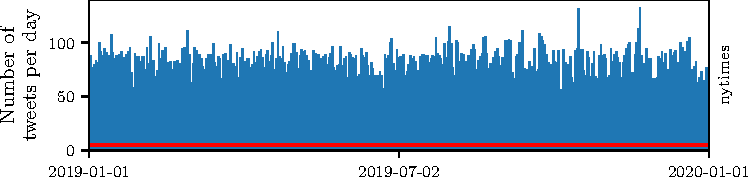
\includegraphics{appendix2/figs/tweet_times/nytimes.pdf}
	\captionof{figure}{Twitter activity over 2019 for `The New York Times'.
		Twitter handle is `nytimes' with 44800317 followers and 31029 total tweets in 2019. }
\end{center}



\begin{center}
	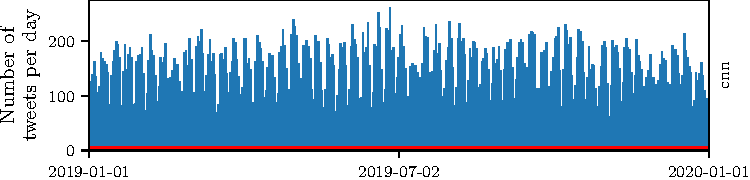
\includegraphics{appendix2/figs/tweet_times/cnn.pdf}
	\captionof{figure}{Twitter activity over 2019 for `CNN'.
		Twitter handle is `cnn' with 44153462 followers and 57155 total tweets in 2019. }
\end{center}



\begin{center}
	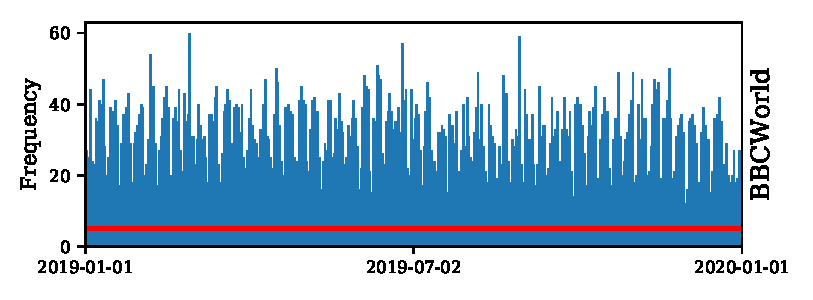
\includegraphics{appendix2/figs/tweet_times/BBCWorld.pdf}
	\captionof{figure}{Twitter activity over 2019 for `BBC News (World)'.
		Twitter handle is `BBCWorld' with 26446876 followers and 11679 total tweets in 2019. }
\end{center}



\begin{center}
	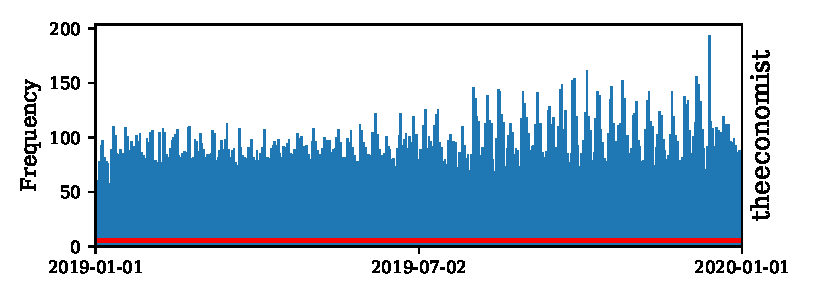
\includegraphics{appendix2/figs/tweet_times/theeconomist.pdf}
	\captionof{figure}{Twitter activity over 2019 for `The Economist'.
		Twitter handle is `theeconomist' with 24239639 followers and 35771 total tweets in 2019. }
\end{center}



\begin{center}
	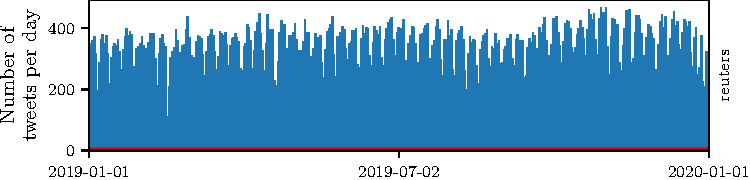
\includegraphics{appendix2/figs/tweet_times/reuters.pdf}
	\captionof{figure}{Twitter activity over 2019 for `Reuters'.
		Twitter handle is `reuters' with 21042215 followers and 128448 total tweets in 2019. }
\end{center}



\begin{center}
	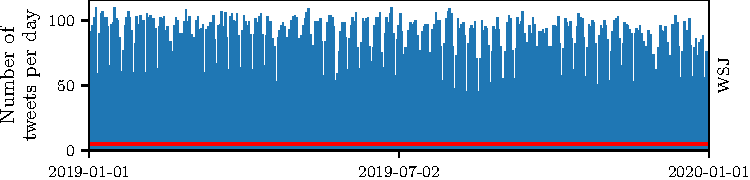
\includegraphics{appendix2/figs/tweet_times/WSJ.pdf}
	\captionof{figure}{Twitter activity over 2019 for `The Wall Street Journal'.
		Twitter handle is `WSJ' with 17139922 followers and 32151 total tweets in 2019. }
\end{center}



\begin{center}
	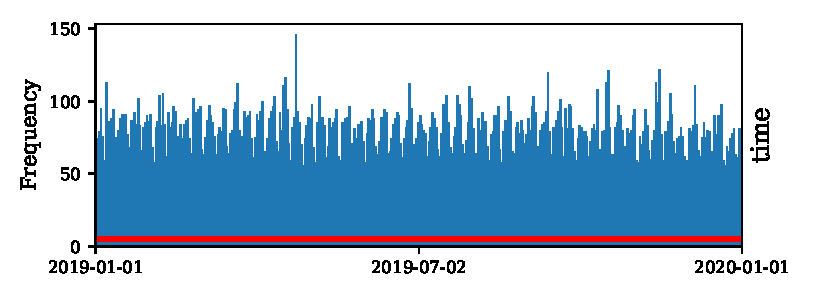
\includegraphics{appendix2/figs/tweet_times/time.pdf}
	\captionof{figure}{Twitter activity over 2019 for `TIME'.
		Twitter handle is `time' with 16512854 followers and 29631 total tweets in 2019. }
\end{center}



\begin{center}
	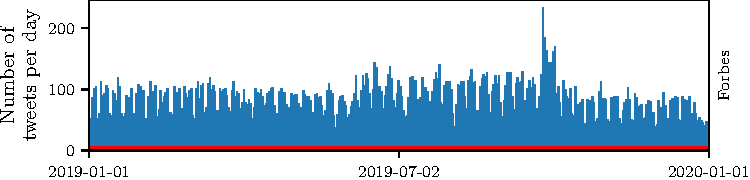
\includegraphics{appendix2/figs/tweet_times/Forbes.pdf}
	\captionof{figure}{Twitter activity over 2019 for `Forbes'.
		Twitter handle is `Forbes' with 15736852 followers and 31940 total tweets in 2019. }
\end{center}



\begin{center}
	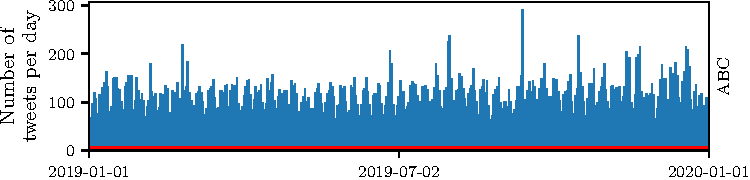
\includegraphics{appendix2/figs/tweet_times/ABC.pdf}
	\captionof{figure}{Twitter activity over 2019 for `ABC News'.
		Twitter handle is `ABC' with 14804638 followers and 44149 total tweets in 2019. }
\end{center}



\begin{center}
	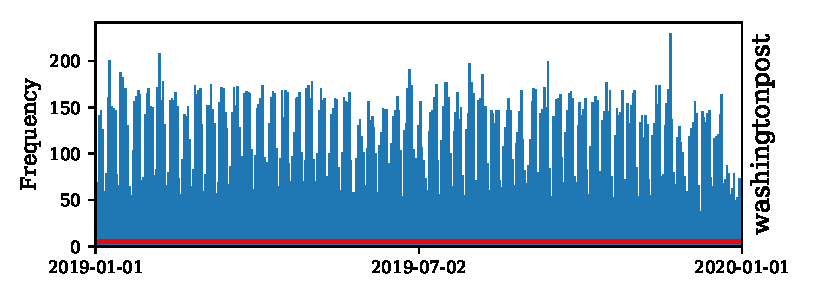
\includegraphics{appendix2/figs/tweet_times/washingtonpost.pdf}
	\captionof{figure}{Twitter activity over 2019 for `The Washington Post'.
		Twitter handle is `washingtonpost' with 14644580 followers and 45043 total tweets in 2019. }
\end{center}



\begin{center}
	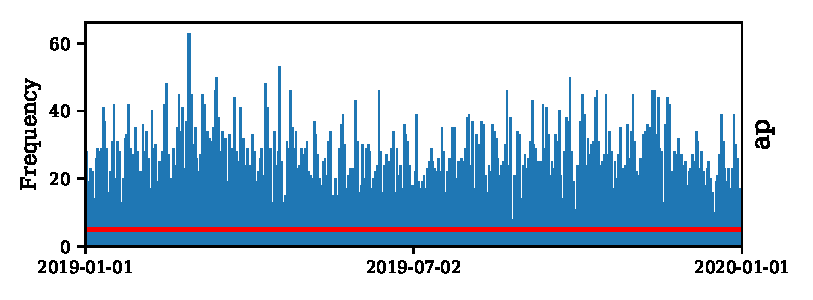
\includegraphics{appendix2/figs/tweet_times/ap.pdf}
	\captionof{figure}{Twitter activity over 2019 for `The Associated Press'.
		Twitter handle is `ap' with 13671750 followers and 10214 total tweets in 2019. }
\end{center}



\begin{center}
	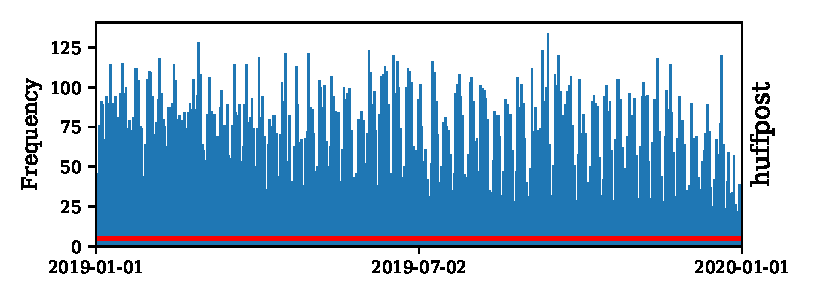
\includegraphics{appendix2/figs/tweet_times/huffpost.pdf}
	\captionof{figure}{Twitter activity over 2019 for `HuffPost'.
		Twitter handle is `huffpost' with 11472382 followers and 27622 total tweets in 2019. }
\end{center}



\begin{center}
	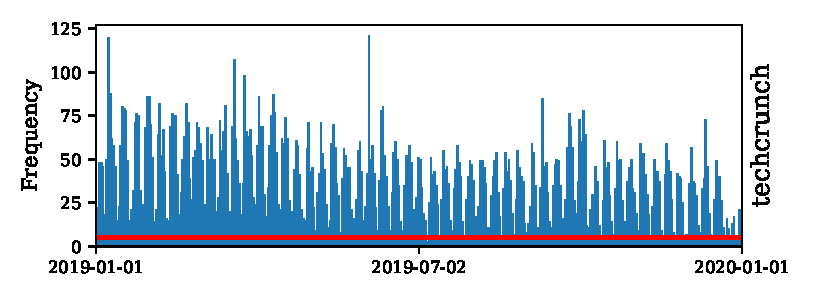
\includegraphics{appendix2/figs/tweet_times/techcrunch.pdf}
	\captionof{figure}{Twitter activity over 2019 for `TechCrunch'.
		Twitter handle is `techcrunch' with 10124437 followers and 14348 total tweets in 2019. }
\end{center}



\begin{center}
	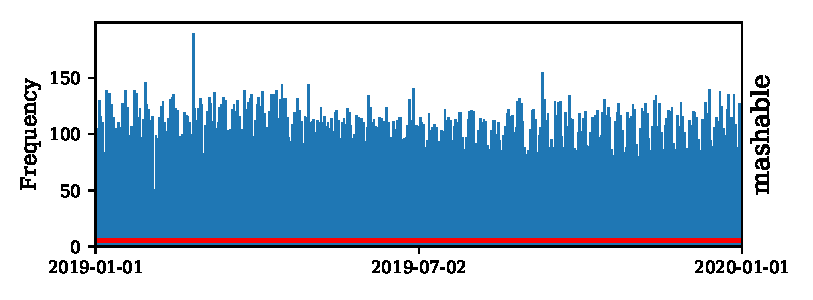
\includegraphics{appendix2/figs/tweet_times/mashable.pdf}
	\captionof{figure}{Twitter activity over 2019 for `Mashable'.
		Twitter handle is `mashable' with 9809420 followers and 40854 total tweets in 2019. }
\end{center}



\begin{center}
	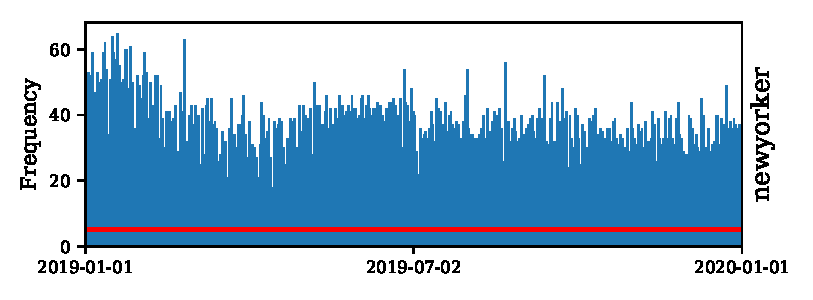
\includegraphics{appendix2/figs/tweet_times/newyorker.pdf}
	\captionof{figure}{Twitter activity over 2019 for `The New Yorker'.
		Twitter handle is `newyorker' with 8774527 followers and 13948 total tweets in 2019. }
\end{center}



\begin{center}
	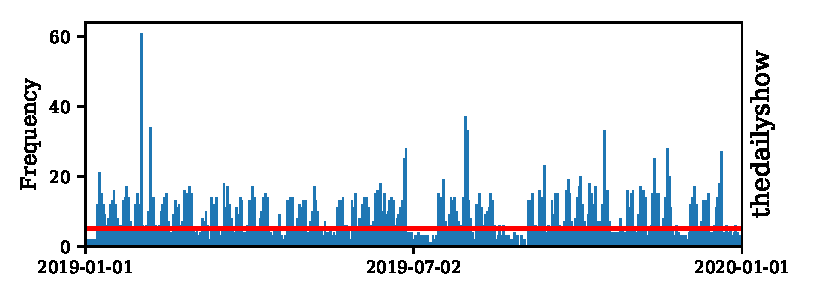
\includegraphics{appendix2/figs/tweet_times/thedailyshow.pdf}
	\captionof{figure}{Twitter activity over 2019 for `The Daily Show'.
		Twitter handle is `thedailyshow' with 8256511 followers and 3386 total tweets in 2019. }
\end{center}



\begin{center}
	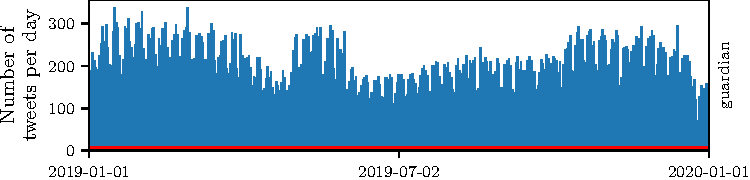
\includegraphics{appendix2/figs/tweet_times/guardian.pdf}
	\captionof{figure}{Twitter activity over 2019 for `The Guardian'.
		Twitter handle is `guardian' with 8243012 followers and 77532 total tweets in 2019. }
\end{center}



\begin{center}
	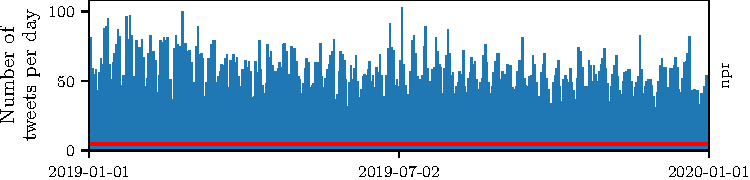
\includegraphics{appendix2/figs/tweet_times/npr.pdf}
	\captionof{figure}{Twitter activity over 2019 for `NPR'.
		Twitter handle is `npr' with 7959364 followers and 21236 total tweets in 2019. }
\end{center}



\begin{center}
	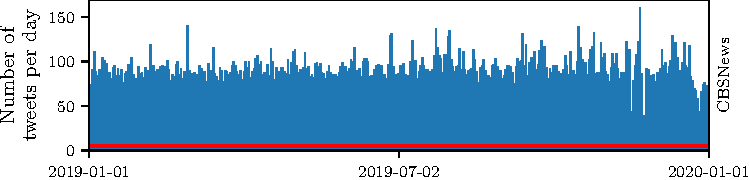
\includegraphics{appendix2/figs/tweet_times/CBSNews.pdf}
	\captionof{figure}{Twitter activity over 2019 for `CBS News'.
		Twitter handle is `CBSNews' with 7078950 followers and 34060 total tweets in 2019. }
\end{center}



\begin{center}
	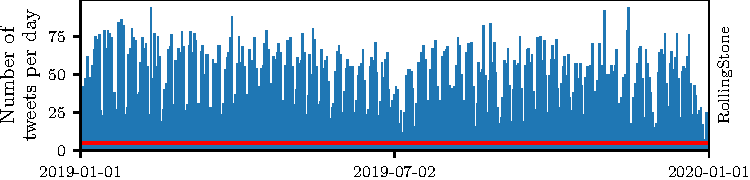
\includegraphics{appendix2/figs/tweet_times/RollingStone.pdf}
	\captionof{figure}{Twitter activity over 2019 for `Rolling Stone'.
		Twitter handle is `RollingStone' with 6295950 followers and 18571 total tweets in 2019. }
\end{center}



\begin{center}
	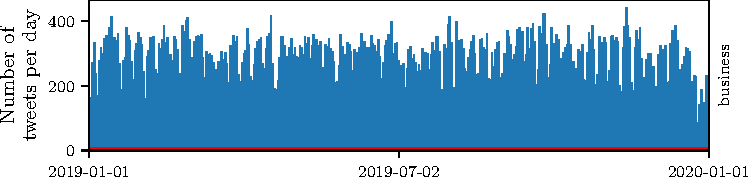
\includegraphics{appendix2/figs/tweet_times/business.pdf}
	\captionof{figure}{Twitter activity over 2019 for `Bloomberg'.
		Twitter handle is `business' with 5790419 followers and 109367 total tweets in 2019. }
\end{center}



\begin{center}
	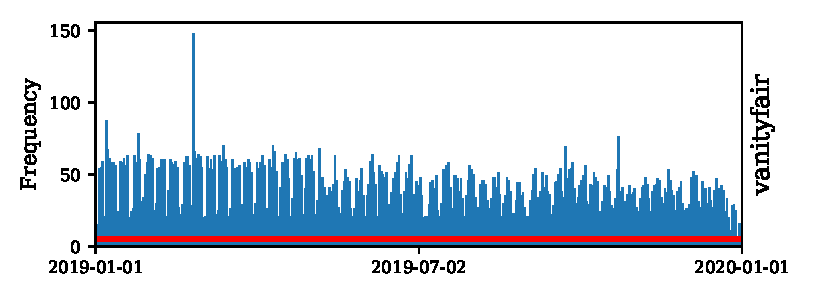
\includegraphics{appendix2/figs/tweet_times/vanityfair.pdf}
	\captionof{figure}{Twitter activity over 2019 for `VANITY FAIR'.
		Twitter handle is `vanityfair' with 4887894 followers and 15585 total tweets in 2019. }
\end{center}



\begin{center}
	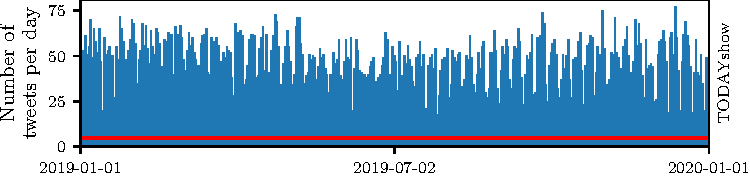
\includegraphics{appendix2/figs/tweet_times/TODAYshow.pdf}
	\captionof{figure}{Twitter activity over 2019 for `TODAY'.
		Twitter handle is `TODAYshow' with 4282063 followers and 17678 total tweets in 2019. }
\end{center}



\begin{center}
	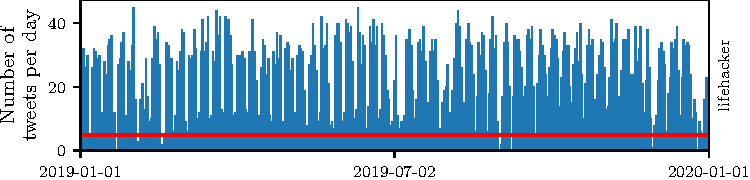
\includegraphics{appendix2/figs/tweet_times/lifehacker.pdf}
	\captionof{figure}{Twitter activity over 2019 for `Lifehacker'.
		Twitter handle is `lifehacker' with 4153410 followers and 9026 total tweets in 2019. }
\end{center}



\begin{center}
	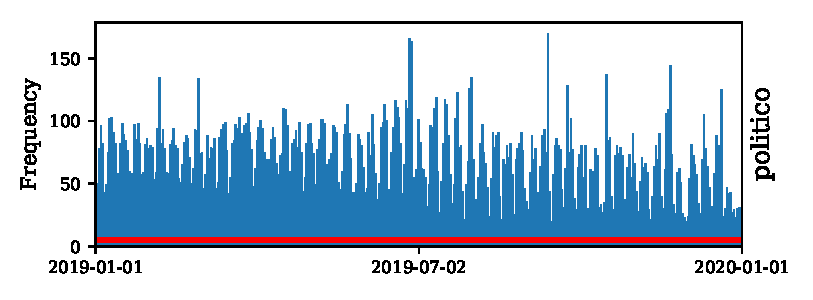
\includegraphics{appendix2/figs/tweet_times/politico.pdf}
	\captionof{figure}{Twitter activity over 2019 for `POLITICO'.
		Twitter handle is `politico' with 4016243 followers and 25742 total tweets in 2019. }
\end{center}



\begin{center}
	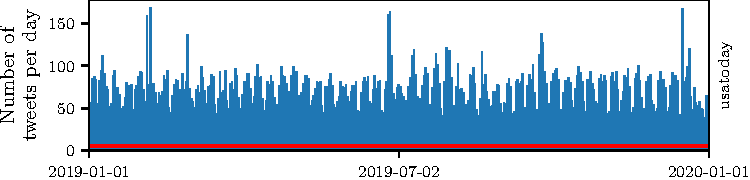
\includegraphics{appendix2/figs/tweet_times/usatoday.pdf}
	\captionof{figure}{Twitter activity over 2019 for `USA TODAY'.
		Twitter handle is `usatoday' with 3949159 followers and 27303 total tweets in 2019. }
\end{center}



\begin{center}
	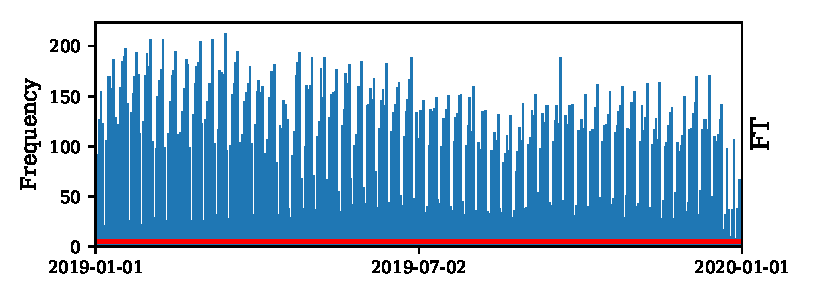
\includegraphics{appendix2/figs/tweet_times/FT.pdf}
	\captionof{figure}{Twitter activity over 2019 for `Financial Times'.
		Twitter handle is `FT' with 3806483 followers and 41030 total tweets in 2019. }
\end{center}



\begin{center}
	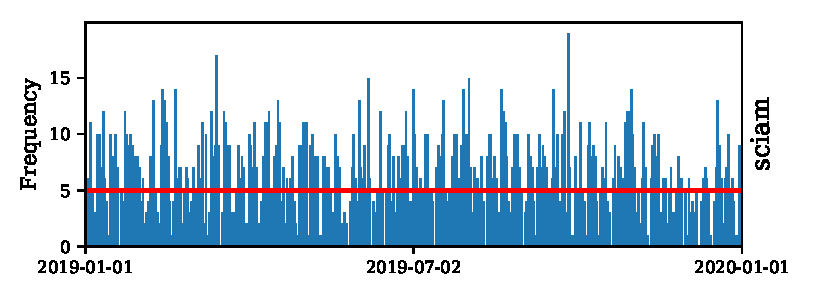
\includegraphics{appendix2/figs/tweet_times/sciam.pdf}
	\captionof{figure}{Twitter activity over 2019 for `Scientific American'.
		Twitter handle is `sciam' with 3805593 followers and 2335 total tweets in 2019. }
\end{center}



\begin{center}
	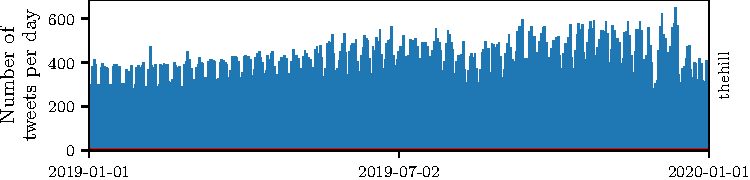
\includegraphics{appendix2/figs/tweet_times/thehill.pdf}
	\captionof{figure}{Twitter activity over 2019 for `The Hill'.
		Twitter handle is `thehill' with 3501890 followers and 157172 total tweets in 2019. }
\end{center}



\begin{center}
	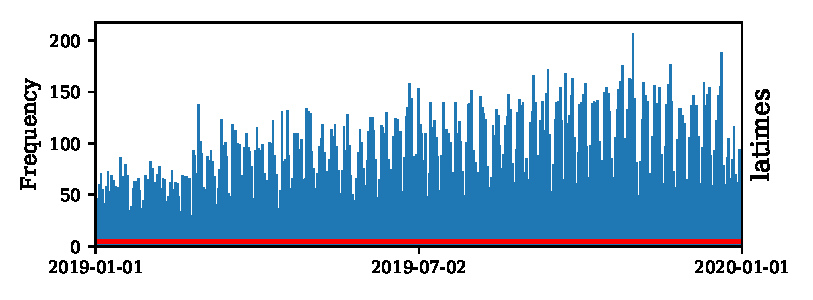
\includegraphics{appendix2/figs/tweet_times/latimes.pdf}
	\captionof{figure}{Twitter activity over 2019 for `Los Angeles Times'.
		Twitter handle is `latimes' with 3473994 followers and 35341 total tweets in 2019. }
\end{center}



\begin{center}
	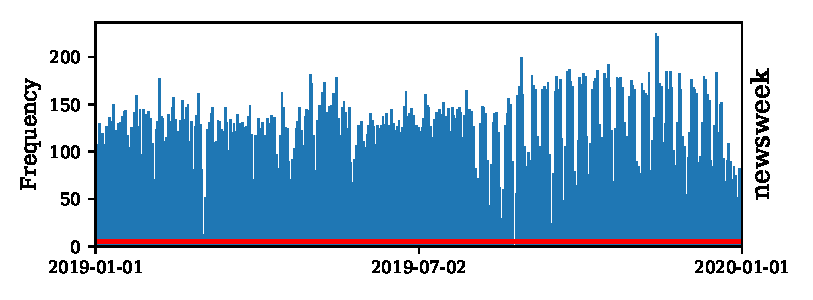
\includegraphics{appendix2/figs/tweet_times/newsweek.pdf}
	\captionof{figure}{Twitter activity over 2019 for `Newsweek'.
		Twitter handle is `newsweek' with 3407905 followers and 46922 total tweets in 2019. }
\end{center}



\begin{center}
	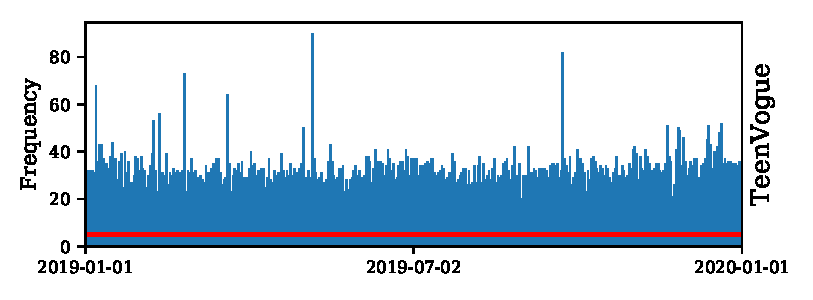
\includegraphics{appendix2/figs/tweet_times/TeenVogue.pdf}
	\captionof{figure}{Twitter activity over 2019 for `Teen Vogue'.
		Twitter handle is `TeenVogue' with 3358001 followers and 12270 total tweets in 2019. }
\end{center}



\begin{center}
	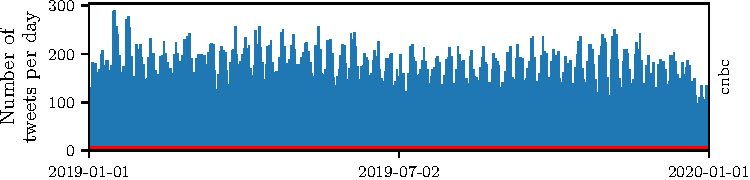
\includegraphics{appendix2/figs/tweet_times/cnbc.pdf}
	\captionof{figure}{Twitter activity over 2019 for `CNBC'.
		Twitter handle is `cnbc' with 3355408 followers and 66578 total tweets in 2019. }
\end{center}



\begin{center}
	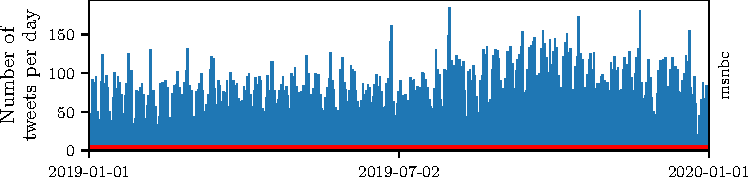
\includegraphics{appendix2/figs/tweet_times/msnbc.pdf}
	\captionof{figure}{Twitter activity over 2019 for `MSNBC'.
		Twitter handle is `msnbc' with 2870702 followers and 32699 total tweets in 2019. }
\end{center}



\begin{center}
	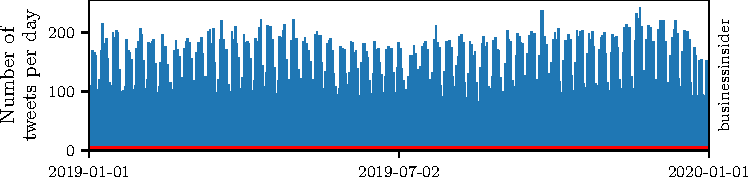
\includegraphics{appendix2/figs/tweet_times/businessinsider.pdf}
	\captionof{figure}{Twitter activity over 2019 for `Business Insider'.
		Twitter handle is `businessinsider' with 2790009 followers and 57915 total tweets in 2019. }
\end{center}



\begin{center}
	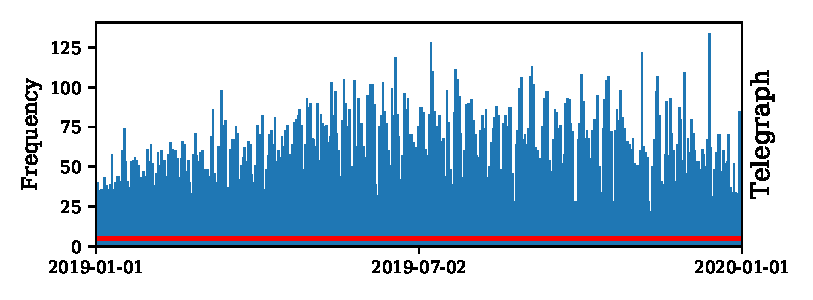
\includegraphics{appendix2/figs/tweet_times/Telegraph.pdf}
	\captionof{figure}{Twitter activity over 2019 for `The Telegraph'.
		Twitter handle is `Telegraph' with 2774439 followers and 24235 total tweets in 2019. }
\end{center}



\begin{center}
	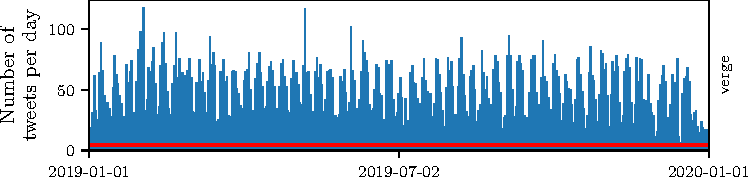
\includegraphics{appendix2/figs/tweet_times/verge.pdf}
	\captionof{figure}{Twitter activity over 2019 for `The Verge'.
		Twitter handle is `verge' with 2613577 followers and 19096 total tweets in 2019. }
\end{center}



\begin{center}
	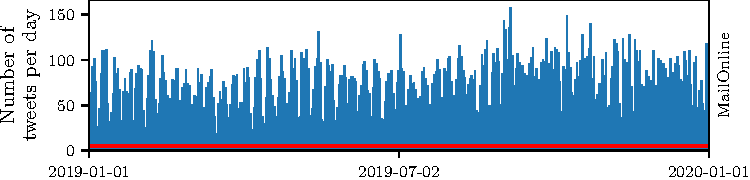
\includegraphics{appendix2/figs/tweet_times/MailOnline.pdf}
	\captionof{figure}{Twitter activity over 2019 for `Daily Mail Online'.
		Twitter handle is `MailOnline' with 2437611 followers and 28671 total tweets in 2019. }
\end{center}



\begin{center}
	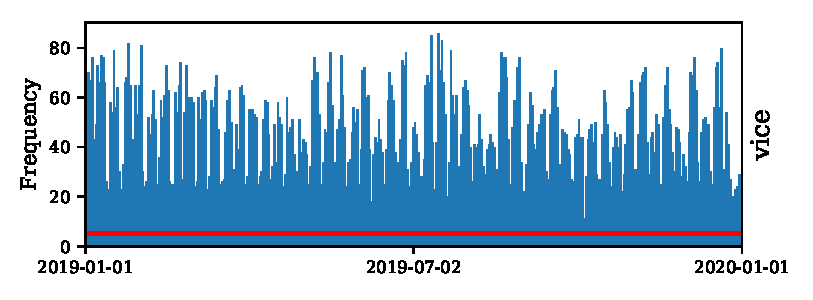
\includegraphics{appendix2/figs/tweet_times/vice.pdf}
	\captionof{figure}{Twitter activity over 2019 for `VICE'.
		Twitter handle is `vice' with 2000034 followers and 17195 total tweets in 2019. }
\end{center}



\begin{center}
	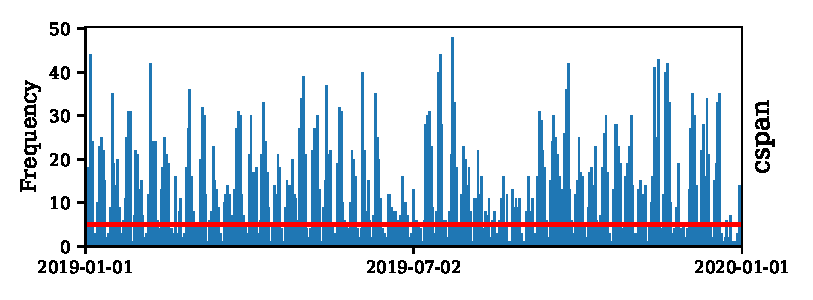
\includegraphics{appendix2/figs/tweet_times/cspan.pdf}
	\captionof{figure}{Twitter activity over 2019 for `CSPAN'.
		Twitter handle is `cspan' with 1989017 followers and 5022 total tweets in 2019. }
\end{center}



\begin{center}
	\includegraphics{appendix2/figs/tweet_times/theatlantic.pdf}
	\captionof{figure}{Twitter activity over 2019 for `The Atlantic'.
		Twitter handle is `theatlantic' with 1850164 followers and 15100 total tweets in 2019. }
\end{center}



\begin{center}
	\includegraphics{appendix2/figs/tweet_times/NYMag.pdf}
	\captionof{figure}{Twitter activity over 2019 for `New York Magazine'.
		Twitter handle is `NYMag' with 1800255 followers and 19072 total tweets in 2019. }
\end{center}



\begin{center}
	\includegraphics{appendix2/figs/tweet_times/slate.pdf}
	\captionof{figure}{Twitter activity over 2019 for `Slate'.
		Twitter handle is `slate' with 1792093 followers and 58598 total tweets in 2019. }
\end{center}



\begin{center}
	\includegraphics{appendix2/figs/tweet_times/AJENews.pdf}
	\captionof{figure}{Twitter activity over 2019 for `Al Jazeera News'.
		Twitter handle is `AJENews' with 1573047 followers and 11252 total tweets in 2019. }
\end{center}



\begin{center}
	\includegraphics{appendix2/figs/tweet_times/nypost.pdf}
	\captionof{figure}{Twitter activity over 2019 for `New York Post'.
		Twitter handle is `nypost' with 1543609 followers and 79771 total tweets in 2019. }
\end{center}



\begin{center}
	\includegraphics{appendix2/figs/tweet_times/BuzzFeedNews.pdf}
	\captionof{figure}{Twitter activity over 2019 for `BuzzFeed News'.
		Twitter handle is `BuzzFeedNews' with 1338555 followers and 19705 total tweets in 2019. }
\end{center}



\begin{center}
	\includegraphics{appendix2/figs/tweet_times/BreitbartNews.pdf}
	\captionof{figure}{Twitter activity over 2019 for `Breitbart News'.
		Twitter handle is `BreitbartNews' with 1225203 followers and 17501 total tweets in 2019. }
\end{center}



\begin{center}
	\includegraphics{appendix2/figs/tweet_times/YahooNews.pdf}
	\captionof{figure}{Twitter activity over 2019 for `Yahoo News'.
		Twitter handle is `YahooNews' with 1106092 followers and 19781 total tweets in 2019. }
\end{center}



\begin{center}
	\includegraphics{appendix2/figs/tweet_times/chicagotribune.pdf}
	\captionof{figure}{Twitter activity over 2019 for `Chicago Tribune'.
		Twitter handle is `chicagotribune' with 1099101 followers and 22994 total tweets in 2019. }
\end{center}



\begin{center}
	\includegraphics{appendix2/figs/tweet_times/ajc.pdf}
	\captionof{figure}{Twitter activity over 2019 for `AJC'.
		Twitter handle is `ajc' with 1045546 followers and 27978 total tweets in 2019. }
\end{center}



\begin{center}
	\includegraphics{appendix2/figs/tweet_times/NewsHour.pdf}
	\captionof{figure}{Twitter activity over 2019 for `PBS NewsHour'.
		Twitter handle is `NewsHour' with 1036993 followers and 16189 total tweets in 2019. }
\end{center}



\begin{center}
	\includegraphics{appendix2/figs/tweet_times/salon.pdf}
	\captionof{figure}{Twitter activity over 2019 for `Salon'.
		Twitter handle is `salon' with 976078 followers and 11614 total tweets in 2019. }
\end{center}



\begin{center}
	\includegraphics{appendix2/figs/tweet_times/voxdotcom.pdf}
	\captionof{figure}{Twitter activity over 2019 for `Vox'.
		Twitter handle is `voxdotcom' with 891290 followers and 17574 total tweets in 2019. }
\end{center}



\begin{center}
	\includegraphics{appendix2/figs/tweet_times/propublica.pdf}
	\captionof{figure}{Twitter activity over 2019 for `ProPublica'.
		Twitter handle is `propublica' with 833038 followers and 6458 total tweets in 2019. }
\end{center}



\begin{center}
	\includegraphics{appendix2/figs/tweet_times/motherjones.pdf}
	\captionof{figure}{Twitter activity over 2019 for `Mother Jones'.
		Twitter handle is `motherjones' with 809121 followers and 16447 total tweets in 2019. }
\end{center}



\begin{center}
	\includegraphics{appendix2/figs/tweet_times/bostonglobe.pdf}
	\captionof{figure}{Twitter activity over 2019 for `The Boston Globe'.
		Twitter handle is `bostonglobe' with 756522 followers and 49224 total tweets in 2019. }
\end{center}



\begin{center}
	\includegraphics{appendix2/figs/tweet_times/theintercept.pdf}
	\captionof{figure}{Twitter activity over 2019 for `The Intercept'.
		Twitter handle is `theintercept' with 753001 followers and 6642 total tweets in 2019. }
\end{center}



\begin{center}
	\includegraphics{appendix2/figs/tweet_times/nydailynews.pdf}
	\captionof{figure}{Twitter activity over 2019 for `New York Daily News'.
		Twitter handle is `nydailynews' with 728512 followers and 28682 total tweets in 2019. }
\end{center}



\begin{center}
	\includegraphics{appendix2/figs/tweet_times/ForeignAffairs.pdf}
	\captionof{figure}{Twitter activity over 2019 for `Foreign Affairs'.
		Twitter handle is `ForeignAffairs' with 724994 followers and 11964 total tweets in 2019. }
\end{center}



\begin{center}
	\includegraphics{appendix2/figs/tweet_times/nytopinion.pdf}
	\captionof{figure}{Twitter activity over 2019 for `New York Times Opinion'.
		Twitter handle is `nytopinion' with 718663 followers and 25402 total tweets in 2019. }
\end{center}



\begin{center}
	\includegraphics{appendix2/figs/tweet_times/democracynow.pdf}
	\captionof{figure}{Twitter activity over 2019 for `Democracy Now!'.
		Twitter handle is `democracynow' with 710714 followers and 9453 total tweets in 2019. }
\end{center}



\begin{center}
	\includegraphics{appendix2/figs/tweet_times/theblaze.pdf}
	\captionof{figure}{Twitter activity over 2019 for `TheBlaze'.
		Twitter handle is `theblaze' with 706991 followers and 13121 total tweets in 2019. }
\end{center}



\begin{center}
	\includegraphics{appendix2/figs/tweet_times/DailyCaller.pdf}
	\captionof{figure}{Twitter activity over 2019 for `Daily Caller'.
		Twitter handle is `DailyCaller' with 579741 followers and 34716 total tweets in 2019. }
\end{center}



\begin{center}
	\includegraphics{appendix2/figs/tweet_times/TheRoot.pdf}
	\captionof{figure}{Twitter activity over 2019 for `The Root'.
		Twitter handle is `TheRoot' with 525879 followers and 6994 total tweets in 2019. }
\end{center}



\begin{center}
	\includegraphics{appendix2/figs/tweet_times/upworthy.pdf}
	\captionof{figure}{Twitter activity over 2019 for `Upworthy'.
		Twitter handle is `upworthy' with 511090 followers and 1472 total tweets in 2019. }
\end{center}



\begin{center}
	\includegraphics{appendix2/figs/tweet_times/OANN.pdf}
	\captionof{figure}{Twitter activity over 2019 for `One America News'.
		Twitter handle is `OANN' with 510392 followers and 6108 total tweets in 2019. }
\end{center}



\begin{center}
	\includegraphics{appendix2/figs/tweet_times/Suntimes.pdf}
	\captionof{figure}{Twitter activity over 2019 for `Chicago Sun-Times'.
		Twitter handle is `Suntimes' with 505161 followers and 15976 total tweets in 2019. }
\end{center}



\begin{center}
	\includegraphics{appendix2/figs/tweet_times/sfgate.pdf}
	\captionof{figure}{Twitter activity over 2019 for `SFGate'.
		Twitter handle is `sfgate' with 477782 followers and 17838 total tweets in 2019. }
\end{center}



\begin{center}
	\includegraphics{appendix2/figs/tweet_times/MiamiHerald.pdf}
	\captionof{figure}{Twitter activity over 2019 for `Miami Herald'.
		Twitter handle is `MiamiHerald' with 450869 followers and 19290 total tweets in 2019. }
\end{center}



\begin{center}
	\includegraphics{appendix2/figs/tweet_times/Jerusalem_Post.pdf}
	\captionof{figure}{Twitter activity over 2019 for `The Jerusalem Post'.
		Twitter handle is `Jerusalem\_Post' with 445004 followers and 29868 total tweets in 2019. }
\end{center}



\begin{center}
	\includegraphics{appendix2/figs/tweet_times/esquire.pdf}
	\captionof{figure}{Twitter activity over 2019 for `Esquire'.
		Twitter handle is `esquire' with 418881 followers and 12817 total tweets in 2019. }
\end{center}



\begin{center}
	\includegraphics{appendix2/figs/tweet_times/qz.pdf}
	\captionof{figure}{Twitter activity over 2019 for `Quartz'.
		Twitter handle is `qz' with 384220 followers and 28604 total tweets in 2019. }
\end{center}



\begin{center}
	\includegraphics{appendix2/figs/tweet_times/WashTimes.pdf}
	\captionof{figure}{Twitter activity over 2019 for `The Washington Times'.
		Twitter handle is `WashTimes' with 372421 followers and 34635 total tweets in 2019. }
\end{center}



\begin{center}
	\includegraphics{appendix2/figs/tweet_times/rollcall.pdf}
	\captionof{figure}{Twitter activity over 2019 for `Roll Call'.
		Twitter handle is `rollcall' with 361580 followers and 10157 total tweets in 2019. }
\end{center}



\begin{center}
	\includegraphics{appendix2/figs/tweet_times/realdailywire.pdf}
	\captionof{figure}{Twitter activity over 2019 for `The Daily Wire'.
		Twitter handle is `realdailywire' with 361505 followers and 26385 total tweets in 2019. }
\end{center}



\begin{center}
	\includegraphics{appendix2/figs/tweet_times/NRO.pdf}
	\captionof{figure}{Twitter activity over 2019 for `National Review'.
		Twitter handle is `NRO' with 336300 followers and 16572 total tweets in 2019. }
\end{center}



\begin{center}
	\includegraphics{appendix2/figs/tweet_times/axios.pdf}
	\captionof{figure}{Twitter activity over 2019 for `Axios'.
		Twitter handle is `axios' with 315533 followers and 19184 total tweets in 2019. }
\end{center}



\begin{center}
	\includegraphics{appendix2/figs/tweet_times/statesman.pdf}
	\captionof{figure}{Twitter activity over 2019 for `Austin Statesman'.
		Twitter handle is `statesman' with 300429 followers and 9562 total tweets in 2019. }
\end{center}



\begin{center}
	\includegraphics{appendix2/figs/tweet_times/dailykos.pdf}
	\captionof{figure}{Twitter activity over 2019 for `Daily Kos'.
		Twitter handle is `dailykos' with 280636 followers and 12636 total tweets in 2019. }
\end{center}



\begin{center}
	\includegraphics{appendix2/figs/tweet_times/reason.pdf}
	\captionof{figure}{Twitter activity over 2019 for `reason'.
		Twitter handle is `reason' with 242262 followers and 7939 total tweets in 2019. }
\end{center}



\begin{center}
	\includegraphics{appendix2/figs/tweet_times/mercnews.pdf}
	\captionof{figure}{Twitter activity over 2019 for `Mercury News'.
		Twitter handle is `mercnews' with 241228 followers and 36535 total tweets in 2019. }
\end{center}



\begin{center}
	\includegraphics{appendix2/figs/tweet_times/jacobinmag.pdf}
	\captionof{figure}{Twitter activity over 2019 for `Jacobin'.
		Twitter handle is `jacobinmag' with 241092 followers and 8579 total tweets in 2019. }
\end{center}



\begin{center}
	\includegraphics{appendix2/figs/tweet_times/sciencedaily.pdf}
	\captionof{figure}{Twitter activity over 2019 for `ScienceDaily'.
		Twitter handle is `sciencedaily' with 240013 followers and 1243 total tweets in 2019. }
\end{center}



\begin{center}
	\includegraphics{appendix2/figs/tweet_times/LasVegasSun.pdf}
	\captionof{figure}{Twitter activity over 2019 for `Las Vegas Sun'.
		Twitter handle is `LasVegasSun' with 238797 followers and 8233 total tweets in 2019. }
\end{center}



\begin{center}
	\includegraphics{appendix2/figs/tweet_times/grist.pdf}
	\captionof{figure}{Twitter activity over 2019 for `grist'.
		Twitter handle is `grist' with 230344 followers and 6438 total tweets in 2019. }
\end{center}



\begin{center}
	\includegraphics{appendix2/figs/tweet_times/sacbee_news.pdf}
	\captionof{figure}{Twitter activity over 2019 for `The Sacramento Bee'.
		Twitter handle is `sacbee\_news' with 219066 followers and 22511 total tweets in 2019. }
\end{center}



\begin{center}
	\includegraphics{appendix2/figs/tweet_times/redstate.pdf}
	\captionof{figure}{Twitter activity over 2019 for `RedState'.
		Twitter handle is `redstate' with 218545 followers and 19778 total tweets in 2019. }
\end{center}



\begin{center}
	\includegraphics{appendix2/figs/tweet_times/FDRLST.pdf}
	\captionof{figure}{Twitter activity over 2019 for `The Federalist'.
		Twitter handle is `FDRLST' with 217053 followers and 5830 total tweets in 2019. }
\end{center}



\begin{center}
	\includegraphics{appendix2/figs/tweet_times/ocregister.pdf}
	\captionof{figure}{Twitter activity over 2019 for `O.C. Register'.
		Twitter handle is `ocregister' with 212517 followers and 23872 total tweets in 2019. }
\end{center}



\begin{center}
	\includegraphics{appendix2/figs/tweet_times/sfweekly.pdf}
	\captionof{figure}{Twitter activity over 2019 for `SF Weekly'.
		Twitter handle is `sfweekly' with 210524 followers and 4438 total tweets in 2019. }
\end{center}



\begin{center}
	\includegraphics{appendix2/figs/tweet_times/rawstory.pdf}
	\captionof{figure}{Twitter activity over 2019 for `Raw Story'.
		Twitter handle is `rawstory' with 205992 followers and 29702 total tweets in 2019. }
\end{center}



\begin{center}
	\includegraphics{appendix2/figs/tweet_times/dcexaminer.pdf}
	\captionof{figure}{Twitter activity over 2019 for `Washington Examiner'.
		Twitter handle is `dcexaminer' with 198229 followers and 61833 total tweets in 2019. }
\end{center}



\begin{center}
	\includegraphics{appendix2/figs/tweet_times/observer.pdf}
	\captionof{figure}{Twitter activity over 2019 for `OBSERVER'.
		Twitter handle is `observer' with 195067 followers and 5856 total tweets in 2019. }
\end{center}



\begin{center}
	\includegraphics{appendix2/figs/tweet_times/sfchronicle.pdf}
	\captionof{figure}{Twitter activity over 2019 for `San Francisco Chronicle'.
		Twitter handle is `sfchronicle' with 189685 followers and 18021 total tweets in 2019. }
\end{center}



\begin{center}
	\includegraphics{appendix2/figs/tweet_times/KSLcom.pdf}
	\captionof{figure}{Twitter activity over 2019 for `KSL'.
		Twitter handle is `KSLcom' with 179424 followers and 11881 total tweets in 2019. }
\end{center}



\begin{center}
	\includegraphics{appendix2/figs/tweet_times/truthout.pdf}
	\captionof{figure}{Twitter activity over 2019 for `Truthout'.
		Twitter handle is `truthout' with 170572 followers and 7806 total tweets in 2019. }
\end{center}



\begin{center}
	\includegraphics{appendix2/figs/tweet_times/newrepublic.pdf}
	\captionof{figure}{Twitter activity over 2019 for `The New Republic'.
		Twitter handle is `newrepublic' with 167916 followers and 10725 total tweets in 2019. }
\end{center}



\begin{center}
	\includegraphics{appendix2/figs/tweet_times/IBDinvestors.pdf}
	\captionof{figure}{Twitter activity over 2019 for `Investors.com'.
		Twitter handle is `IBDinvestors' with 167242 followers and 2469 total tweets in 2019. }
\end{center}



\begin{center}
	\includegraphics{appendix2/figs/tweet_times/PittsburghPG.pdf}
	\captionof{figure}{Twitter activity over 2019 for `Pittsburgh Post-Gazette'.
		Twitter handle is `PittsburghPG' with 166684 followers and 24711 total tweets in 2019. }
\end{center}



\begin{center}
	\includegraphics{appendix2/figs/tweet_times/memphisnews.pdf}
	\captionof{figure}{Twitter activity over 2019 for `Commercial Appeal'.
		Twitter handle is `memphisnews' with 162002 followers and 15885 total tweets in 2019. }
\end{center}



\begin{center}
	\includegraphics{appendix2/figs/tweet_times/Mediaite.pdf}
	\captionof{figure}{Twitter activity over 2019 for `Mediaite'.
		Twitter handle is `Mediaite' with 159980 followers and 14030 total tweets in 2019. }
\end{center}



\begin{center}
	\includegraphics{appendix2/figs/tweet_times/townhallcom.pdf}
	\captionof{figure}{Twitter activity over 2019 for `Townhall.com'.
		Twitter handle is `townhallcom' with 152082 followers and 10452 total tweets in 2019. }
\end{center}



\begin{center}
	\includegraphics{appendix2/figs/tweet_times/usnews.pdf}
	\captionof{figure}{Twitter activity over 2019 for `U.S. News'.
		Twitter handle is `usnews' with 150674 followers and 12827 total tweets in 2019. }
\end{center}



\begin{center}
	\includegraphics{appendix2/figs/tweet_times/alternet.pdf}
	\captionof{figure}{Twitter activity over 2019 for `AlterNet'.
		Twitter handle is `alternet' with 139194 followers and 7156 total tweets in 2019. }
\end{center}



\begin{center}
	\includegraphics{appendix2/figs/tweet_times/nationaljournal.pdf}
	\captionof{figure}{Twitter activity over 2019 for `National Journal'.
		Twitter handle is `nationaljournal' with 133097 followers and 1424 total tweets in 2019. }
\end{center}



\begin{center}
	\includegraphics{appendix2/figs/tweet_times/theweek.pdf}
	\captionof{figure}{Twitter activity over 2019 for `The Week'.
		Twitter handle is `theweek' with 129703 followers and 9031 total tweets in 2019. }
\end{center}



\begin{center}
	\includegraphics{appendix2/figs/tweet_times/CBNNews.pdf}
	\captionof{figure}{Twitter activity over 2019 for `CBN News'.
		Twitter handle is `CBNNews' with 128487 followers and 15627 total tweets in 2019. }
\end{center}



\begin{center}
	\includegraphics{appendix2/figs/tweet_times/IBTimes.pdf}
	\captionof{figure}{Twitter activity over 2019 for `Intl. Business Times'.
		Twitter handle is `IBTimes' with 123358 followers and 11519 total tweets in 2019. }
\end{center}



\begin{center}
	\includegraphics{appendix2/figs/tweet_times/cnsnews.pdf}
	\captionof{figure}{Twitter activity over 2019 for `CNSNews.com'.
		Twitter handle is `cnsnews' with 119236 followers and 9035 total tweets in 2019. }
\end{center}



\begin{center}
	\includegraphics{appendix2/figs/tweet_times/RTDNEWS.pdf}
	\captionof{figure}{Twitter activity over 2019 for `Times-Dispatch'.
		Twitter handle is `RTDNEWS' with 116510 followers and 7018 total tweets in 2019. }
\end{center}



\begin{center}
	\includegraphics{appendix2/figs/tweet_times/FreeBeacon.pdf}
	\captionof{figure}{Twitter activity over 2019 for `Free Beacon'.
		Twitter handle is `FreeBeacon' with 110634 followers and 9091 total tweets in 2019. }
\end{center}



\begin{center}
	\includegraphics{appendix2/figs/tweet_times/bostonherald.pdf}
	\captionof{figure}{Twitter activity over 2019 for `Boston Herald'.
		Twitter handle is `bostonherald' with 105046 followers and 12550 total tweets in 2019. }
\end{center}



\begin{center}
	\includegraphics{appendix2/figs/tweet_times/newsmax.pdf}
	\captionof{figure}{Twitter activity over 2019 for `Newsmax'.
		Twitter handle is `newsmax' with 100437 followers and 3825 total tweets in 2019. }
\end{center}



\begin{center}
	\includegraphics{appendix2/figs/tweet_times/curaffairs.pdf}
	\captionof{figure}{Twitter activity over 2019 for `Current Affairs'.
		Twitter handle is `curaffairs' with 99136 followers and 2188 total tweets in 2019. }
\end{center}



\begin{center}
	\includegraphics{appendix2/figs/tweet_times/DeseretNews.pdf}
	\captionof{figure}{Twitter activity over 2019 for `Deseret News'.
		Twitter handle is `DeseretNews' with 97060 followers and 15087 total tweets in 2019. }
\end{center}



\begin{center}
	\includegraphics{appendix2/figs/tweet_times/WSJopinion.pdf}
	\captionof{figure}{Twitter activity over 2019 for `WSJ Editorial Page'.
		Twitter handle is `WSJopinion' with 96734 followers and 4990 total tweets in 2019. }
\end{center}



\begin{center}
	\includegraphics{appendix2/figs/tweet_times/bustle.pdf}
	\captionof{figure}{Twitter activity over 2019 for `Bustle'.
		Twitter handle is `bustle' with 96170 followers and 1504 total tweets in 2019. }
\end{center}



\begin{center}
	\includegraphics{appendix2/figs/tweet_times/courierjournal.pdf}
	\captionof{figure}{Twitter activity over 2019 for `Courier Journal'.
		Twitter handle is `courierjournal' with 88551 followers and 13988 total tweets in 2019. }
\end{center}



\begin{center}
	\includegraphics{appendix2/figs/tweet_times/PressHerald.pdf}
	\captionof{figure}{Twitter activity over 2019 for `Portland Press Herald'.
		Twitter handle is `PressHerald' with 85834 followers and 6372 total tweets in 2019. }
\end{center}



\begin{center}
	\includegraphics{appendix2/figs/tweet_times/DefenseOne.pdf}
	\captionof{figure}{Twitter activity over 2019 for `Defense One'.
		Twitter handle is `DefenseOne' with 81992 followers and 6892 total tweets in 2019. }
\end{center}



\begin{center}
	\includegraphics{appendix2/figs/tweet_times/The_Nation.pdf}
	\captionof{figure}{Twitter activity over 2019 for `The Nation'.
		Twitter handle is `The\_Nation' with 78860 followers and 13048 total tweets in 2019. }
\end{center}



\begin{center}
	\includegraphics{appendix2/figs/tweet_times/csmonitor.pdf}
	\captionof{figure}{Twitter activity over 2019 for `The Christian Science Monitor'.
		Twitter handle is `csmonitor' with 75406 followers and 5676 total tweets in 2019. }
\end{center}



\begin{center}
	\includegraphics{appendix2/figs/tweet_times/ArkansasOnline.pdf}
	\captionof{figure}{Twitter activity over 2019 for `AR Democrat-Gazette'.
		Twitter handle is `ArkansasOnline' with 74177 followers and 10951 total tweets in 2019. }
\end{center}



\begin{center}
	\includegraphics{appendix2/figs/tweet_times/indyweek.pdf}
	\captionof{figure}{Twitter activity over 2019 for `INDY Week'.
		Twitter handle is `indyweek' with 73802 followers and 4175 total tweets in 2019. }
\end{center}



\begin{center}
	\includegraphics{appendix2/figs/tweet_times/PoliticusUSA.pdf}
	\captionof{figure}{Twitter activity over 2019 for `PoliticusUSA'.
		Twitter handle is `PoliticusUSA' with 72856 followers and 7253 total tweets in 2019. }
\end{center}



\begin{center}
	\includegraphics{appendix2/figs/tweet_times/Dailysignal.pdf}
	\captionof{figure}{Twitter activity over 2019 for `The Daily Signal'.
		Twitter handle is `Dailysignal' with 68024 followers and 6740 total tweets in 2019. }
\end{center}



\begin{center}
	\includegraphics{appendix2/figs/tweet_times/PJMedia_com.pdf}
	\captionof{figure}{Twitter activity over 2019 for `PJ Media'.
		Twitter handle is `PJMedia\_com' with 66324 followers and 5666 total tweets in 2019. }
\end{center}



\begin{center}
	\includegraphics{appendix2/figs/tweet_times/delcotimes.pdf}
	\captionof{figure}{Twitter activity over 2019 for `Delco Times'.
		Twitter handle is `delcotimes' with 64714 followers and 3302 total tweets in 2019. }
\end{center}



\begin{center}
	\includegraphics{appendix2/figs/tweet_times/Daily_Press.pdf}
	\captionof{figure}{Twitter activity over 2019 for `Daily Press'.
		Twitter handle is `Daily\_Press' with 61225 followers and 3512 total tweets in 2019. }
\end{center}



\begin{center}
	\includegraphics{appendix2/figs/tweet_times/yesmagazine.pdf}
	\captionof{figure}{Twitter activity over 2019 for `YES! Magazine'.
		Twitter handle is `yesmagazine' with 60455 followers and 4679 total tweets in 2019. }
\end{center}



\begin{center}
	\includegraphics{appendix2/figs/tweet_times/SpokesmanReview.pdf}
	\captionof{figure}{Twitter activity over 2019 for `SpokesmanReview'.
		Twitter handle is `SpokesmanReview' with 58352 followers and 4113 total tweets in 2019. }
\end{center}



\begin{center}
	\includegraphics{appendix2/figs/tweet_times/TDOnline.pdf}
	\captionof{figure}{Twitter activity over 2019 for `Tallahassee Democrat'.
		Twitter handle is `TDOnline' with 53700 followers and 15098 total tweets in 2019. }
\end{center}



\begin{center}
	\includegraphics{appendix2/figs/tweet_times/TheKoreaHerald.pdf}
	\captionof{figure}{Twitter activity over 2019 for `The Korea Herald'.
		Twitter handle is `TheKoreaHerald' with 53517 followers and 8730 total tweets in 2019. }
\end{center}



\begin{center}
	\includegraphics{appendix2/figs/tweet_times/michigandaily.pdf}
	\captionof{figure}{Twitter activity over 2019 for `The Michigan Daily'.
		Twitter handle is `michigandaily' with 50748 followers and 2041 total tweets in 2019. }
\end{center}



\begin{center}
	\includegraphics{appendix2/figs/tweet_times/CivilBeat.pdf}
	\captionof{figure}{Twitter activity over 2019 for `Honolulu Civil Beat'.
		Twitter handle is `CivilBeat' with 50503 followers and 1837 total tweets in 2019. }
\end{center}



\begin{center}
	\includegraphics{appendix2/figs/tweet_times/TheLibRepublic.pdf}
	\captionof{figure}{Twitter activity over 2019 for `Libertarian Republic'.
		Twitter handle is `TheLibRepublic' with 47475 followers and 1145 total tweets in 2019. }
\end{center}



\begin{center}
	\includegraphics{appendix2/figs/tweet_times/amconmag.pdf}
	\captionof{figure}{Twitter activity over 2019 for `The American Conservative'.
		Twitter handle is `amconmag' with 46189 followers and 25197 total tweets in 2019. }
\end{center}



\begin{center}
	\includegraphics{appendix2/figs/tweet_times/amspectator.pdf}
	\captionof{figure}{Twitter activity over 2019 for `The American Spectator'.
		Twitter handle is `amspectator' with 45877 followers and 1915 total tweets in 2019. }
\end{center}



\begin{center}
	\includegraphics{appendix2/figs/tweet_times/redandblack.pdf}
	\captionof{figure}{Twitter activity over 2019 for `The Red \& Black'.
		Twitter handle is `redandblack' with 42735 followers and 7663 total tweets in 2019. }
\end{center}



\begin{center}
	\includegraphics{appendix2/figs/tweet_times/kqednews.pdf}
	\captionof{figure}{Twitter activity over 2019 for `KQED News'.
		Twitter handle is `kqednews' with 41720 followers and 8655 total tweets in 2019. }
\end{center}



\begin{center}
	\includegraphics{appendix2/figs/tweet_times/idsnews.pdf}
	\captionof{figure}{Twitter activity over 2019 for `Indiana Daily Student'.
		Twitter handle is `idsnews' with 41621 followers and 3867 total tweets in 2019. }
\end{center}



\begin{center}
	\includegraphics{appendix2/figs/tweet_times/wgbh.pdf}
	\captionof{figure}{Twitter activity over 2019 for `WGBH'.
		Twitter handle is `wgbh' with 39971 followers and 2211 total tweets in 2019. }
\end{center}



\begin{center}
	\includegraphics{appendix2/figs/tweet_times/WestJournalism.pdf}
	\captionof{figure}{Twitter activity over 2019 for `The Western Journal'.
		Twitter handle is `WestJournalism' with 38478 followers and 7114 total tweets in 2019. }
\end{center}



\begin{center}
	\includegraphics{appendix2/figs/tweet_times/Commentary.pdf}
	\captionof{figure}{Twitter activity over 2019 for `Commentary Magazine'.
		Twitter handle is `Commentary' with 35704 followers and 1337 total tweets in 2019. }
\end{center}



\begin{center}
	\includegraphics{appendix2/figs/tweet_times/DailyProgress.pdf}
	\captionof{figure}{Twitter activity over 2019 for `The Daily Progress'.
		Twitter handle is `DailyProgress' with 35506 followers and 6856 total tweets in 2019. }
\end{center}



\begin{center}
	\includegraphics{appendix2/figs/tweet_times/vtdigger.pdf}
	\captionof{figure}{Twitter activity over 2019 for `VTDigger'.
		Twitter handle is `vtdigger' with 32820 followers and 5671 total tweets in 2019. }
\end{center}



\begin{center}
	\includegraphics{appendix2/figs/tweet_times/bgdailynews.pdf}
	\captionof{figure}{Twitter activity over 2019 for `BG Daily News'.
		Twitter handle is `bgdailynews' with 22341 followers and 7686 total tweets in 2019. }
\end{center}



\begin{center}
	\includegraphics{appendix2/figs/tweet_times/TimesCall.pdf}
	\captionof{figure}{Twitter activity over 2019 for `Longmont Times-Call'.
		Twitter handle is `TimesCall' with 21077 followers and 3858 total tweets in 2019. }
\end{center}



\begin{center}
	\includegraphics{appendix2/figs/tweet_times/thedailynu.pdf}
	\captionof{figure}{Twitter activity over 2019 for `The Daily Northwestern'.
		Twitter handle is `thedailynu' with 20357 followers and 4580 total tweets in 2019. }
\end{center}



\begin{center}
	\includegraphics{appendix2/figs/tweet_times/rightsidenews.pdf}
	\captionof{figure}{Twitter activity over 2019 for `Right Side News: Breaking News \& Opinion'.
		Twitter handle is `rightsidenews' with 17600 followers and 4033 total tweets in 2019. }
\end{center}



\begin{center}
	\includegraphics{appendix2/figs/tweet_times/wfae.pdf}
	\captionof{figure}{Twitter activity over 2019 for `WFAE'.
		Twitter handle is `wfae' with 17385 followers and 4317 total tweets in 2019. }
\end{center}



\begin{center}
	\includegraphics{appendix2/figs/tweet_times/CollegeFix.pdf}
	\captionof{figure}{Twitter activity over 2019 for `The College Fix'.
		Twitter handle is `CollegeFix' with 15289 followers and 4094 total tweets in 2019. }
\end{center}



\begin{center}
	\includegraphics{appendix2/figs/tweet_times/DukeChronicle.pdf}
	\captionof{figure}{Twitter activity over 2019 for `The Chronicle'.
		Twitter handle is `DukeChronicle' with 15207 followers and 1537 total tweets in 2019. }
\end{center}



\begin{center}
	\includegraphics{appendix2/figs/tweet_times/calmatters.pdf}
	\captionof{figure}{Twitter activity over 2019 for `CalMatters'.
		Twitter handle is `calmatters' with 15069 followers and 3247 total tweets in 2019. }
\end{center}

 
%%!TEX root = ../thesis.tex
\chapter{Tandem queue processes \label{app:tand}}

 

\backmatter
% Add the bibliography to the table of contents
\addcontentsline{toc}{chapter}{Bibliography}

% What style to use and what file to use for the bibliography
\bibliographystyle{agsm}
\bibliography{bibliography/thesis}
\bibliography{bibliography/Data}

\end{document}

